%----------
%   CONFIGURACIÓN DEL DOCUMENTO
%----------

\documentclass[12pt]{report}

\usepackage[a4paper, vmargin=2.5cm, hmargin=3cm]{geometry}
\renewcommand{\baselinestretch}{1.15}
\parskip=6pt

\usepackage[table]{xcolor}
\definecolor{azulUC3M}{RGB}{0,0,102}
\definecolor{gray97}{gray}{.97}
\definecolor{gray75}{gray}{.75}
\definecolor{gray45}{gray}{.45}

\usepackage[a-1b]{pdfx}
\usepackage{hyperref}
\hypersetup{colorlinks=true, linkcolor=black, urlcolor=blue}

\usepackage{amsmath,amssymb,amsfonts,amsthm}
\usepackage{txfonts}
\usepackage[T1]{fontenc}
\usepackage[utf8]{inputenc}
\usepackage[spanish, es-tabla]{babel}
\usepackage[babel, spanish=spanish]{csquotes}
\AtBeginEnvironment{quote}{\small}

\usepackage{fancyhdr}
\pagestyle{fancy}
\fancyhf{}
\renewcommand{\headrulewidth}{0pt}
\rfoot{\thepage}
\fancypagestyle{plain}{\pagestyle{fancy}}

\usepackage{titlesec}
\usepackage{titletoc}
\titleformat{\chapter}[block]
{\large\bfseries\filcenter}{\thechapter.}{5pt}{\MakeUppercase}{}
\titlespacing{\chapter}{0pt}{0pt}{*3}
\titlecontents{chapter}[0pt]{}
{\contentsmargin{0pt}\thecontentslabel.\enspace\uppercase}
{\contentsmargin{0pt}\uppercase}
{\titlerule*[.7pc]{.}\contentspage}

\titleformat{\section}{\bfseries}{\thesection.}{5pt}{}
\titlecontents{section}[5pt]{}
{\contentsmargin{0pt}\thecontentslabel.\enspace}
{\contentsmargin{0pt}}
{\titlerule*[.7pc]{.}\contentspage}

\titleformat{\subsection}{\normalsize\bfseries}{\thesubsection.}{5pt}{}
\titlecontents{subsection}[10pt]{}
{\contentsmargin{0pt}\thecontentslabel.\enspace}
{\contentsmargin{0pt}}
{\titlerule*[.7pc]{.}\contentspage}

\usepackage{multirow}
\usepackage{caption}
\usepackage{floatrow}
\usepackage{array}
\newcolumntype{P}[1]{>{\centering\arraybackslash}p{#1}}
\DeclareCaptionFormat{upper}{#1#2\uppercase{#3}\par}

\captionsetup*[table]{
    format=upper, name=TABLA, justification=centering,
    labelsep=period, width=.75\linewidth, labelfont=small, font=small
}

\usepackage{graphicx}
\graphicspath{{imagenes/}}

\captionsetup[figure]{
    format=hang, name=Fig., singlelinecheck=off,
    labelsep=period, labelfont=small, font=small
}

\usepackage{chngcntr}
\counterwithout{footnote}{chapter}

\usepackage{listings}
\lstdefinestyle{estilo}{
    frame=Ltb, framerule=0pt, aboveskip=0.5cm,
    framextopmargin=3pt, framexbottommargin=3pt, framexleftmargin=0.4cm,
    framesep=0pt, rulesep=.4pt, backgroundcolor=\color{gray97},
    rulesepcolor=\color{black},
    basicstyle=\ttfamily\footnotesize, keywordstyle=\bfseries,
    stringstyle=\ttfamily, showstringspaces=false,
    commentstyle=\color{gray45},
    numbers=left, numbersep=15pt, numberstyle=\tiny,
    numberfirstline=false, breaklines=true, xleftmargin=\parindent
}
\captionsetup*[lstlisting]{font=small, labelsep=period}
\lstset{style=estilo}
\renewcommand{\lstlistingname}{\uppercase{Código}}

\usepackage[backend=biber, style=ieee, isbn=false, sortcites,
    maxbibnames=6, minbibnames=1]{biblatex}
\DefineBibliographyStrings{spanish}{andothers={et\addabbrvspace al\adddot}}
\DefineBibliographyStrings{spanish}{url={\adddot\space[En línea]\adddot\space Disponible en:}}
\DefineBibliographyStrings{spanish}{urlseen={Acceso:}}
\DefineBibliographyStrings{spanish}{pages={pp\adddot}, page={p.\adddot}}
\addbibresource{referencias.bib}


%-------------
%   DOCUMENTO
%-------------

\begin{document}
\pagenumbering{roman}

%----------
%   PORTADA
%----------
\begin{titlepage}
    \begin{sffamily}
    \color{azulUC3M}
    \begin{center}
        \begin{figure}[H]
            \makebox[\textwidth][c]{\includegraphics[width=16cm]{logo_UC3M.png}}
        \end{figure}
        \vspace{2.5cm}
        \begin{Large}
            Grado en Ingeniería Informática\\
            2024-2025\\
            \vspace{2cm}
            \textsl{Trabajo Fin de Grado}
            \bigskip
        \end{Large}
        {\Huge ``Análisis de sesgos relacionados con la discapacidad en modelos de IA Generativa en español''}\\
        \vspace*{0.5cm}
        \rule{10.5cm}{0.1mm}\\
        \vspace*{0.9cm}
        {\LARGE Alejandro López Sancho}\\
        \vspace*{1cm}
        \begin{Large}
            Tutor\\
            Lourdes Moreno López\\
            \vspace{0.5cm}
            Leganés, junio de 2025\\
        \end{Large}
    \end{center}
    \vfill
    \color{black}
    \includegraphics[width=4.2cm]{creativecommons.png}\\
    Esta obra se encuentra sujeta a la licencia Creative Commons\\
    \textbf{Reconocimiento - No Comercial - Sin Obra Derivada}
    \end{sffamily}
\end{titlepage}

\newpage
\thispagestyle{empty}
\mbox{}

%----------
%   RESUMEN
%----------
\renewcommand\abstractname{\large\bfseries\filcenter\uppercase{Resumen}}
\begin{abstract}
\thispagestyle{plain}
\setcounter{page}{3}

Los modelos de lenguaje de gran escala (LLMs) se utilizan de forma creciente en contextos que afectan directamente a la vida de las personas: asistencia sanitaria, empleo, educación y servicios públicos. Sin embargo, existe evidencia creciente de que estos modelos pueden generar respuestas sesgadas cuando las consultas incluyen referencias a grupos sociales específicos. El colectivo de personas con discapacidad representa una de las poblaciones más vulnerables a este tipo de sesgo, y el estudio de este fenómeno en lengua española ha recibido escasa atención en la literatura científica.

Este Trabajo Fin de Grado diseña, implementa y ejecuta un marco experimental reproducible para analizar si los modelos de IA generativa en español modifican de forma sistemática su comportamiento cuando una consulta incorpora una referencia explícita a la discapacidad. Para ello, se construye un dataset original de 100 plantillas de prompts contrafactuales, organizadas en cinco dominios temáticos (empleo, educación, salud, administración y ocio) y enriquecidas con siete tipos de discapacidad, generando un total de 800 prompts finales.

El experimento se ejecuta sobre cuatro modelos: \textit{Llama 3.1 8B Instruct} (Meta), \textit{RigoChat 7B v2} (IIC), \textit{Gemini 2.5 Flash} (Google) y \textit{Salamandra 7B Instruct} (BSC-LT). Las respuestas de cada modelo se evalúan mediante tres métricas automáticas complementarias: análisis de sentimiento con el modelo \textit{robertuito} de pysentimiento, evaluación mediante un juez LLM basado en una rúbrica de cinco dimensiones (relevancia, exactitud, utilidad, tono respetuoso y ausencia de estereotipo), y diferencia de extensión entre las respuestas neutra y con discapacidad.

Los resultados muestran que los tres modelos locales evaluados (Llama 3.1 8B Instruct, RigoChat 7B v2 y Salamandra 7B Instruct) presentan sesgo detectable en más del 85\% de los prompts, frente al 11\% de Gemini 2.5 Flash. La dimensión más afectada en todos los modelos locales es la ausencia de estereotipo, con caídas medias de entre $-1{,}41$ y $-1{,}44$ puntos sobre 5. Las discapacidades cognitiva e intelectual resultan las más estigmatizadas, y el dominio de empleo el más vulnerable. Estos resultados demuestran que la especialización en español no garantiza un comportamiento más equitativo, y que el sesgo hacia las personas con discapacidad es un problema real y cuantificable en los modelos de IA generativa actuales.

\textbf{Palabras clave:} sesgos en IA, modelos de lenguaje, discapacidad, prompts contrafactuales, evaluación automática, español, análisis de sentimiento, LLM-as-judge.

\vfill
\end{abstract}

\newpage
\thispagestyle{empty}
\mbox{}

%----------
%   DEDICATORIA
%----------
\chapter*{Dedicatoria}
\setcounter{page}{5}

% [Alejandro: escribe aquí tu dedicatoria]

\vfill

\newpage
\thispagestyle{empty}
\mbox{}

%----------
%   ÍNDICES
%----------
\tableofcontents
\thispagestyle{fancy}

\newpage
\thispagestyle{empty}
\mbox{}

\listoffigures
\thispagestyle{fancy}

\newpage
\thispagestyle{empty}
\mbox{}

\listoftables
\thispagestyle{fancy}

\newpage
\thispagestyle{empty}
\mbox{}


%----------
%   MEMORIA
%----------
\clearpage
\pagenumbering{arabic}

% ============================================================
\chapter{Introducción}
% ============================================================

\section{Contexto}

En los últimos años, los modelos de lenguaje de gran escala —o LLMs, como se les conoce habitualmente— han pasado a ser una herramienta cotidiana para millones de personas en todo el mundo. Gracias a la arquitectura \textit{transformer} \cite{vaswani2017attention} y a su entrenamiento sobre enormes cantidades de texto, sistemas como GPT-4, Llama o Gemini son capaces de generar texto coherente, responder preguntas, redactar documentos o mantener conversaciones de una forma que hace unos años habría parecido imposible.

Como consecuencia de esto, estos modelos se están integrando en ámbitos que afectan directamente a la vida de las personas: atención sanitaria, educación, servicios públicos, selección de personal o asesoría legal, entre otros. En el contexto del español, esto es especialmente relevante dado que es la segunda lengua más hablada del mundo, y ha surgido un ecosistema propio de modelos orientados específicamente a esta lengua, como RigoChat (desarrollado por el IIC), Salamandra (del Barcelona Supercomputing Center) o ALIA.

El problema es que, junto con todas estas capacidades, los LLMs heredan los sesgos que existen en los datos con los que se han entrenado \cite{navigli2023biases, guo2024bias}. Estos sesgos no siempre son fáciles de detectar: a menudo no se manifiestan como insultos o contenido claramente ofensivo, sino como diferencias sutiles en el tono, la cantidad de información proporcionada o la forma en que se presenta a determinados grupos de personas. El colectivo de personas con discapacidad es uno de los que más pueden verse afectados por este tipo de comportamientos. Según datos del Instituto Nacional de Estadística, en España hay aproximadamente 4,38 millones de personas con algún tipo de discapacidad (cerca del 9,4\% de la población), y a nivel mundial la OMS estima que más de 1.300 millones de personas viven con alguna forma de discapacidad significativa. Si los sistemas de IA que se despliegan para toda la ciudadanía tratan de forma diferente a este colectivo, el impacto puede ser considerable.


\section{Motivación}

La idea de este TFG surge de una combinación de factores que, al juntarse, hacen que el tema resulte especialmente interesante y necesario.

Por un lado, revisando la literatura científica sobre sesgos en LLMs \cite{guo2024bias, navigli2023biases}, nos dimos cuenta de que la inmensa mayoría de los estudios se centran en inglés y en atributos como el género o la etnia. El sesgo hacia las personas con discapacidad está comparativamente muy poco estudiado, y en español prácticamente no existen trabajos al respecto. Hay algunos estudios en inglés que demuestran que los modelos asocian términos de discapacidad con sentimientos negativos \cite{venkit2022disability} o que reproducen estereotipos sutiles hacia este colectivo \cite{gadiraju2023disability}, pero nadie ha explorado si esto ocurre también en los modelos que se están desarrollando específicamente para el español.

Por otro lado, hoy en día es perfectamente posible llevar a cabo este tipo de experimentos de forma rigurosa sin necesitar una infraestructura enorme, gracias a que muchos modelos son de código abierto y se pueden ejecutar en GPUs accesibles. Esto nos permitió diseñar un experimento real, con modelos reales, y no quedarnos en algo meramente teórico.

En definitiva, el trabajo responde a una pregunta que nadie ha respondido todavía para el español: ¿cambian los LLMs su comportamiento cuando una consulta menciona a una persona con discapacidad? Y si cambia, ¿de qué forma?


\section{Problema abordado}

El problema concreto que abordamos en este trabajo es el siguiente: cuando se le pide a un modelo de IA generativa en español que genere un texto, ¿produce respuestas distintas dependiendo de si la consulta menciona o no a una persona con discapacidad? Y si lo hace, ¿en qué sentido cambia esa respuesta?

Lo importante es que este tipo de sesgo —denominado en la literatura sesgo extrínseco o de salida \cite{navigli2023biases}— no tiene por qué manifestarse de forma obvia. El modelo no tiene que insultar a nadie para ser discriminatorio. Lo que los trabajos previos han encontrado \cite{gadiraju2023disability} es que los sesgos suelen ser más sutiles: el modelo puede volverse más paternalista, añadir advertencias innecesarias, reducir el nivel de detalle de su respuesta, o introducir estereotipos de forma implícita. Esto hace que detectarlos sea más difícil y que haga falta ir más allá de un simple detector de toxicidad.


\section{Objetivos}

\subsection{Objetivo general}

El objetivo general de este Trabajo Fin de Grado es diseñar, implementar y evaluar un marco experimental reproducible para analizar posibles sesgos relacionados con la discapacidad en modelos de inteligencia artificial generativa en español, mediante el uso de prompts contrafactuales y la comparación sistemática de las respuestas generadas por distintos modelos.

\subsection{Objetivos específicos}

Los objetivos específicos de este Trabajo Fin de Grado son los siguientes:

\begin{itemize}
    \item Estudiar los fundamentos y trabajos relacionados sobre sesgos en modelos generativos, con especial atención a los sesgos vinculados a la discapacidad.

    \item Definir un diseño experimental basado en prompts contrafactuales que permita comparar respuestas generadas ante consultas neutras y consultas con referencias explícitas a la discapacidad.

    \item Diseñar la arquitectura del pipeline experimental, incluyendo la organización del dataset, la ejecución sobre distintos modelos, el almacenamiento de respuestas y la preparación de los datos para su análisis.

    \item Implementar un proceso reproducible para ejecutar los prompts sobre los modelos seleccionados y conservar las respuestas generadas junto con la información necesaria para su trazabilidad.

    \item Evaluar y comparar los resultados obtenidos mediante una combinación de análisis automático y revisión manual.

    \item Analizar las limitaciones del trabajo y proponer posibles líneas de mejora para futuras ampliaciones.
\end{itemize}


\section{Alcance del trabajo}

El presente trabajo abarca el diseño del dataset de prompts contrafactuales, la implementación del pipeline de ejecución y evaluación, la ejecución del experimento sobre cuatro modelos seleccionados, el análisis automático de las respuestas generadas y la discusión de los resultados obtenidos.

Quedan fuera del alcance de este trabajo los siguientes aspectos: el desarrollo de técnicas de mitigación de sesgos, la evaluación de modelos de generación de imágenes o audio, la generalización de resultados a todos los contextos hispanohablantes (dado que el español presenta variación geográfica y cultural significativa), la validación estadística con evaluadores humanos a gran escala (aunque sí se incluye una revisión manual de una muestra), y el análisis de sesgos en tareas de comprensión lectora o clasificación (el estudio se limita a la generación de texto).


\section{Estructura de la memoria}

El resto de la memoria se organiza del siguiente modo. El capítulo 2 presenta el estado del arte, revisando los conceptos fundamentales sobre modelos de lenguaje de gran escala, los tipos de sesgos identificados en la literatura, los trabajos previos sobre sesgo relacionado con la discapacidad, las metodologías de evaluación disponibles, las técnicas de mitigación propuestas en la literatura y los modelos seleccionados para el estudio. El capítulo 3 describe el análisis del problema y los requisitos del marco experimental. El capítulo 4 presenta el diseño detallado del experimento, incluyendo el dataset, el esquema de almacenamiento y el protocolo de evaluación. El capítulo 5 describe la implementación del pipeline. El capítulo 6 recoge los resultados experimentales y su discusión. El capítulo 7 incluye la planificación, el presupuesto y el impacto del trabajo. El capítulo 8 cierra la memoria con las conclusiones y las líneas de trabajo futuro.


% ============================================================
\chapter{Estado del arte}
% ============================================================

\section{Introducción}

Para poder entender bien el trabajo que se presenta en esta memoria, conviene revisar primero qué se sabe sobre los temas que lo rodean. Este capítulo empieza explicando qué son los modelos de lenguaje de gran escala y cómo funcionan a grandes rasgos, para después centrarse en el problema de los sesgos: de dónde vienen, qué tipos existen y cómo se miden. Se dedica especial atención a los trabajos que han estudiado específicamente los sesgos hacia las personas con discapacidad, que son los más directamente relacionados con este TFG. También se repasan las metodologías de evaluación disponibles, los benchmarks de referencia y las herramientas que se han utilizado para medir el sesgo en este trabajo. El capítulo termina con una descripción de los cuatro modelos seleccionados para el experimento.


\section{Modelos generativos de lenguaje}

Los modelos de lenguaje de gran escala —o LLMs, por sus siglas en inglés— son el tipo de sistema de inteligencia artificial que se analiza en este trabajo. Se trata de redes neuronales entrenadas con cantidades enormes de texto con el objetivo de aprender a generar texto coherente y útil. La arquitectura que los sustenta desde 2017 es el \textit{transformer} \cite{vaswani2017attention}, que introdujo el mecanismo de atención para capturar relaciones entre palabras distantes en una misma secuencia. Este avance resultó clave: permitió escalar los modelos a un número de parámetros antes impensable y obtener una capacidad de generación muy superior a la de las arquitecturas anteriores basadas en redes recurrentes.

El entrenamiento de estos modelos suele dividirse en dos grandes fases. En la primera, llamada \textit{pretraining}, el modelo aprende a predecir el siguiente token de un texto a partir de corpus masivos obtenidos de internet, libros y otras fuentes. El resultado es un modelo con mucho ``conocimiento'' sobre el lenguaje, pero sin orientación concreta hacia ninguna tarea. En la segunda fase, el modelo se ajusta para seguir instrucciones de forma útil y segura, principalmente mediante \textit{fine-tuning} supervisado y aprendizaje por refuerzo a partir de retroalimentación humana (RLHF) \cite{ouyang2022instructgpt}. Esta segunda etapa es especialmente importante desde el punto de vista de los sesgos: si los evaluadores humanos que proporcionan la retroalimentación no son suficientemente diversos o si las directrices de evaluación no contemplan de forma explícita la equidad, el proceso puede consolidar o incluso amplificar sesgos presentes en los datos \cite{guo2024bias}.

En paralelo al desarrollo de modelos multilingües de propósito general, en los últimos años han surgido iniciativas orientadas específicamente al español. El Instituto de Ingeniería del Conocimiento (IIC) ha desarrollado RigoChat \cite{rigochat}, el Barcelona Supercomputing Center (BSC-LT) ha publicado Salamandra \cite{salamandra}, y proyectos como ALIA buscan potenciar el ecosistema de modelos en lengua española. Estos modelos se distinguen de los grandes modelos multilingües por haber puesto un mayor énfasis en la calidad y el volumen de datos en español durante el entrenamiento, lo que en teoría debería resultar en un mejor rendimiento en tareas en castellano. Sin embargo, si esas mejoras también se traducen en un comportamiento más equitativo hacia colectivos como las personas con discapacidad es una pregunta que no tiene una respuesta clara a priori, y que precisamente este trabajo pretende explorar.


\section{Sesgos en modelos de inteligencia artificial}

\subsection{Origen de los sesgos}

Entender de dónde vienen los sesgos en los LLMs es el primer paso para poder evaluarlos y, en su caso, corregirlos. La literatura identifica tres grandes fuentes \cite{navigli2023biases, guo2024bias}. La primera y más obvia son los datos de entrenamiento: si los textos con los que se entrena un modelo contienen estereotipos, asociaciones negativas hacia ciertos grupos o una representación desequilibrada de determinadas poblaciones, el modelo los aprenderá e incorporará a sus salidas. No es algo intencionado, sino una consecuencia directa del hecho de que los modelos aprenden de lo que hay en internet y en los libros, y esos textos reflejan la sociedad con todos sus prejuicios.

La segunda fuente tiene que ver con el proceso de ajuste. Durante el RLHF, personas reales evalúan las respuestas del modelo y deciden cuáles son mejores. Si esos evaluadores tienen sus propios sesgos —algo prácticamente inevitable— o si las instrucciones de evaluación no contemplan explícitamente la equidad hacia todos los grupos, el modelo puede aprender a tratar de forma diferente a personas en función de sus características. Esto es especialmente problemático porque suele pasar de forma no intencionada y es difícil de detectar durante el desarrollo.

Por último, la propia tarea puede desencadenar comportamientos sesgados que no se observan en otros contextos. Un modelo puede comportarse de forma aparentemente neutra en una conversación general y mostrar un sesgo claro cuando se le pide que escriba un correo de rechazo laboral a un candidato con discapacidad.

\subsection{Tipos de sesgos en modelos de lenguaje}

\citeauthor{navigli2023biases} \cite{navigli2023biases} proponen una clasificación bastante completa de los tipos de sesgo que se pueden encontrar en los LLMs. El \textbf{sesgo de representación} es quizás el más estudiado: el modelo asocia sistemáticamente a ciertos grupos con atributos positivos o negativos. El \textbf{sesgo de estereotipo} ocurre cuando el modelo reproduce asociaciones estereotipadas entre grupos y características (por ejemplo, asumir que una persona con discapacidad intelectual no puede tomar decisiones legales). El \textbf{sesgo de framing} se manifiesta cuando la forma de presentar la información sobre un grupo está sesgada aunque el contenido sea técnicamente correcto. Y el \textbf{sesgo de omisión} se da cuando el modelo omite información relevante de forma diferencial: por ejemplo, explicar con mucho detalle cómo acceder a un servicio público cuando el usuario es descrito como una persona sin discapacidad, y dar una respuesta mucho más escueta o condescendiente cuando se menciona que tiene discapacidad.

\subsection{Sesgos intrínsecos y sesgos extrínsecos}

Otra distinción que conviene tener clara es la que separa los sesgos intrínsecos de los extrínsecos, porque determinan qué tipo de experimentos son necesarios para medirlos \cite{navigli2023biases}.

Los \textbf{sesgos intrínsecos} están en las representaciones internas del modelo: en cómo organiza el espacio semántico, qué palabras considera similares o qué asociaciones establece entre conceptos. Se pueden medir con técnicas como WEAT (\textit{Word Embedding Association Test}), que compara la proximidad entre términos demográficos y valorativos en ese espacio. Son interesantes desde un punto de vista teórico, pero no siempre se traducen directamente en comportamientos problemáticos cuando el modelo genera texto.

Los \textbf{sesgos extrínsecos}, en cambio, se manifiestan en las salidas concretas del modelo ante tareas reales. Son los que tienen un impacto más directo en las personas que usan el sistema, y son los que se estudian en este trabajo. El enfoque adoptado aquí —comparar las respuestas ante consultas neutras y consultas con referencia a la discapacidad— es precisamente un método de evaluación extrínseca.


\section{Sesgos relacionados con la discapacidad}

El sesgo hacia las personas con discapacidad en los modelos de lenguaje es un área de investigación relativamente reciente. Aunque el problema lleva años siendo una preocupación en los estudios de accesibilidad e inclusión digital, su análisis específico en LLMs no empezó a recibir atención significativa hasta principios de los años 2020.

Uno de los primeros trabajos sistemáticos en esta línea es el de \citeauthor{venkit2022disability} \cite{venkit2022disability}, que construyeron más de 15.000 frases combinando adjetivos de uso común con términos relacionados con distintos tipos de discapacidad y sin ellos. Los resultados fueron bastante contundentes: todos los modelos analizados asignaban puntuaciones de sentimiento más negativas a las frases que incluían referencias a la discapacidad. En el caso de un modelo preentrenado sobre datos de Twitter, el sesgo llegaba a invertir el sentimiento de la frase —de positivo a negativo— en el 86\% de los casos cuando se añadía un término de discapacidad. Esto sugiere que el sesgo no es un fenómeno marginal sino algo bastante consistente y extendido.

Lo interesante del trabajo de \citeauthor{gadiraju2023disability} \cite{gadiraju2023disability} es que ponen el foco no en las métricas sino en la experiencia real de las personas con discapacidad. Realizaron 19 grupos de discusión con 56 participantes que interactuaron directamente con un modelo de diálogo y luego discutieron sus respuestas. La conclusión más importante de su estudio es que los participantes rara vez encontraron respuestas abiertamente ofensivas o tóxicas, pero sí identificaron formas más sutiles y molestas de sesgo: el modelo tendía a presentarlos como fuente de inspiración para otras personas (\textit{inspiration porn}), a asumir que necesitaban ayuda constante de personas sin discapacidad, o a reproducir estereotipos que habían visto también en medios convencionales. Esto es relevante para este TFG porque muestra que medir sesgo con detectores de toxicidad no es suficiente: hace falta ir más allá.

En 2025 se han publicado varios trabajos más que avanzan en esta dirección. \citeauthor{panda2025accesseval} \cite{panda2025accesseval} proponen \textit{AccessEval}, un benchmark específico para evaluar el sesgo hacia la discapacidad en LLMs que trabaja con 234 consultas neutras y más de 2.000 con discapacidad distribuidas en seis dominios y nueve tipos de discapacidad. Sus resultados confirman que los modelos generan respuestas con más errores factuales, mayor negatividad y más estereotipos cuando las consultas incluyen referencias a la discapacidad. Este trabajo es la referencia metodológica más directa para el presente estudio.

\citeauthor{dash2025leftbehind} \cite{dash2025leftbehind} auditan 17 modelos en cuanto a su capacidad de dar respuestas inclusivas sobre diferentes tipos de discapacidad, y encuentran que los modelos cubren razonablemente bien la discapacidad visual, auditiva y motriz, pero dejan muy atrás a personas con discapacidades del habla, del desarrollo o de salud mental. Este resultado es útil como referencia comparativa para los análisis por tipo de discapacidad de este trabajo.

Más en la línea del dominio de empleo —uno de los cinco dominios que analiza este TFG—, \citeauthor{kamruzzaman2025disclosure} \cite{kamruzzaman2025disclosure} demuestran que revelar información sobre discapacidades en procesos de selección automatizados introduce sesgos discriminatorios sistemáticos. Por su parte, \citeauthor{phutane2025ableist} \cite{phutane2025ableist} introducen el concepto de \textit{capacitismo} (\textit{ableism}) en LLMs y proponen el marco ABLEIST, que identifica cinco tipos específicos de daño hacia personas con discapacidad en escenarios de contratación, incluyendo fenómenos como la superhumanización o el tokenismo.


\section{Evaluación de sesgos mediante prompts contrafactuales}

La metodología sobre la que se apoya todo el diseño experimental de este trabajo es la evaluación mediante pruebas contrafactuales. La idea, en realidad, es bastante intuitiva: si quiero saber si un modelo trata de forma diferente a las personas con discapacidad, lo más directo es presentarle exactamente la misma situación dos veces —una con referencia a la discapacidad y otra sin ella— y comparar las respuestas.

Esta técnica tiene sus raíces en el estudio de sesgos de género en sistemas de procesamiento del lenguaje. \citeauthor{zhao2018winobias} \cite{zhao2018winobias} la aplicaron para demostrar que los sistemas de resolución de correferencias asignaban pronombres de forma estereotipada según la ocupación de las personas en la oración. La adaptación al estudio de sesgos hacia la discapacidad es directa: en lugar de cambiar el género, se cambia (o se introduce) la referencia a un tipo de discapacidad, manteniendo todo lo demás igual.

La principal ventaja de este enfoque es que permite aislar el efecto del atributo sensible estudiado. Si las respuestas del modelo son diferentes entre la versión neutra y la versión con discapacidad, la única explicación posible —dado que todo lo demás es idéntico— es que el modelo está reaccionando de forma diferente ante esa referencia. Esto convierte los resultados en evidencia bastante directa de sesgo, a diferencia de otros métodos que requieren más supuestos. \citeauthor{guo2024bias} \cite{guo2024bias} señalan precisamente el \textit{counterfactual testing} como una de las técnicas más sólidas disponibles para la evaluación extrínseca de sesgos en LLMs.


\section{Benchmarks y trabajos relacionados}

\subsection{Benchmarks generales sobre sesgos}

Existen varios benchmarks que abordan el sesgo en LLMs desde una perspectiva más general, sin centrarse en un grupo demográfico concreto. \textit{BEATS} \cite{beats2025} es uno de los más recientes y completos: evalúa 29 métricas distintas que cubren sesgos demográficos, cognitivos y sociales, razonamiento ético y riesgo de desinformación. Sus resultados muestran que el 37,65\% de las salidas de los modelos más avanzados contienen algún tipo de sesgo, lo que da una idea de la magnitud del problema. \textit{HELM Safety} \cite{helmsafety2024}, desarrollado por el Stanford Center for Research on Foundation Models, ofrece un marco más orientado a la seguridad que evalúa los modelos en múltiples tareas y dimensiones de riesgo.

\subsection{Benchmarks específicos sobre discapacidad}

En el contexto específico de la discapacidad, \textit{AccessEval} \cite{panda2025accesseval} es el benchmark más relevante y el que más influye en el diseño de este trabajo. Para el español, el benchmark \textit{SESGO} \cite{sesgo2025} cubre más de 4.000 prompts con estereotipos de género, raza y clase socioeconómica, aunque no aborda la discapacidad de forma específica. Esta laguna es precisamente uno de los argumentos que justifican el presente trabajo: hasta donde sabemos, no existe ningún benchmark en español centrado en el sesgo hacia la discapacidad.


\section{Métricas y estrategias de evaluación}

\subsection{Métricas automáticas}

Una de las métricas más utilizadas en la literatura para cuantificar el sesgo en las respuestas generadas es el análisis de sentimiento \cite{venkit2022disability, panda2025accesseval}. La idea es sencilla: si el modelo genera respuestas sistemáticamente más negativas cuando se menciona una discapacidad, eso es una señal de sesgo. Para el inglés, herramientas como VADER permiten hacer este análisis de forma rápida, aunque con limitaciones por su naturaleza léxica. Para el español, la opción más adecuada es el modelo \textit{robertuito}, disponible a través de la librería pysentimiento \cite{perez2021pysentimiento}. Se trata de un modelo basado en RoBERTa y entrenado específicamente sobre texto en español, que devuelve probabilidades de sentimiento positivo (POS), negativo (NEG) y neutro (NEU). En este trabajo se utiliza el score $\text{POS} - \text{NEG} \in [-1, 1]$ como indicador cuantitativo del tono de cada respuesta.

Otra métrica relevante es \textit{Regard}, propuesta por \citeauthor{sheng2019regard} \cite{sheng2019regard} para medir específicamente la percepción social hacia grupos demográficos en texto generado. A diferencia del sentimiento general, Regard está pensado para capturar si el texto presenta a un grupo de forma positiva, negativa o neutra, lo que lo hace conceptualmente más adecuado para el estudio del sesgo. Aunque en este trabajo se utiliza el sentimiento como proxy por disponibilidad de modelos en español, la lógica subyacente es la misma que propone Regard.

Por último, la \textbf{diferencia de extensión} es una métrica simple pero que puede ser muy informativa: si el modelo escribe respuestas sistemáticamente más largas o más cortas cuando menciona una discapacidad, podría estar aportando más o menos información de la necesaria, lo que también es una forma de sesgo.

\subsection{Evaluación mediante jueces automáticos}

Hay dimensiones del sesgo —como el paternalismo, la condescendencia o el uso de estereotipos— que son difíciles de capturar con una sola puntuación numérica. Para abordar esto, en los últimos años ha cobrado mucha popularidad el uso de LLMs como evaluadores de las respuestas de otros modelos, lo que se conoce como LLM-as-judge \cite{zheng2023llmjudge}. La idea es pedirle a un modelo de gran capacidad que evalúe una respuesta siguiendo una rúbrica predefinida, de la misma forma que lo haría un evaluador humano.

\citeauthor{zheng2023llmjudge} \cite{zheng2023llmjudge} estudiaron la viabilidad de este enfoque y encontraron que modelos como GPT-4 alcanzan más del 80\% de acuerdo con las preferencias humanas en evaluaciones abiertas. También identificaron algunos sesgos del propio juez —tendencia a preferir respuestas largas, a favorecer su propio estilo— lo que hay que tener en cuenta al interpretar los resultados.

En este trabajo se utiliza Gemini 2.5 Flash como juez, con una rúbrica de cinco dimensiones puntuadas de 1 a 5: relevancia, exactitud, utilidad, tono respetuoso y ausencia de estereotipo. Para minimizar el riesgo de autoevaluación, el juez opera en modo ciego —sin información sobre qué modelo generó la respuesta— y con la función de \textit{thinking} desactivada para obtener salidas más deterministas.

\subsection{Evaluación humana}

Ninguna métrica automática es perfecta para detectar el tipo de sesgo sutil que describen \citeauthor{gadiraju2023disability} \cite{gadiraju2023disability}. Por eso, el protocolo de este trabajo incluye también una revisión manual de una muestra de respuestas. Esta revisión utiliza la misma rúbrica que el juez automático, lo que permite comparar ambas evaluaciones y tener una idea de hasta qué punto el juez LLM es fiable en este contexto concreto.


\section{Técnicas de mitigación de sesgos}

El objetivo de este TFG es la \textit{detección} y cuantificación del sesgo, no su corrección. Sin embargo, revisar las técnicas de mitigación que propone la literatura es importante por dos razones: permite entender qué tipo de intervenciones han podido influir en el comportamiento de los modelos que evaluamos (especialmente en el caso de Gemini 2.5 Flash), y establece el marco de referencia para las propuestas de trabajo futuro que se recogen en el capítulo 8. La literatura agrupa estas técnicas en tres niveles según la fase del ciclo de vida del modelo en la que actúan \cite{navigli2023biases, guo2024bias}.

\subsection{Intervenciones a nivel de datos}

Las técnicas de nivel de datos actúan antes de que el modelo aprenda nada, modificando el corpus de entrenamiento para que el sesgo no llegue a codificarse en los pesos del modelo. Son las más efectivas a largo plazo pero también las más costosas de aplicar, ya que requieren auditar y modificar conjuntos de datos de enormes dimensiones.

En el caso concreto del sesgo hacia la discapacidad, las intervenciones más relevantes son el \textbf{filtrado léxico del corpus}, que consiste en detectar y eliminar términos estigmatizantes o desactualizados (\textit{minusválido}, \textit{retrasado}, \textit{postrado en silla de ruedas}), y el \textbf{balanceo y aumento de datos}, que busca compensar la tendencia de los textos extraídos de internet a asociar la discapacidad con la compasión o la limitación, inyectando intencionalmente textos donde las personas con discapacidad aparecen en roles de liderazgo, autonomía o situaciones cotidianas neutras.

\subsection{Intervenciones a nivel de arquitectura y entrenamiento}

Las técnicas de nivel de arquitectura modifican el propio proceso de aprendizaje del modelo para que, incluso si los datos de entrenamiento contienen sesgos, el modelo no los asimile como reglas válidas. La más relevante para el contexto de este trabajo es la \textbf{equidad contrafactual} (\textit{counterfactual fairness}): entrenar al modelo con el objetivo explícito de producir salidas idénticas independientemente del atributo sensible que aparezca en la entrada. En el dominio de la discapacidad, esto significa que el modelo debería puntuar igual el currículum de un candidato con y sin referencia a su discapacidad, o dar la misma información sobre un trámite administrativo con independencia de si el usuario se identifica como persona con discapacidad.

La otra técnica habitual en este nivel es el \textbf{\textit{fine-tuning} supervisado con datos equilibrados}: partiendo de un modelo base preentrenado, se realiza un ajuste fino con un conjunto de datos pequeño pero cuidadosamente curado, generalmente con la participación de expertos en inclusión y derechos de las personas con discapacidad. Esta es la técnica más accesible computacionalmente para aplicar correcciones específicas sin necesidad de reentrenar el modelo completo.

\subsection{Intervenciones a nivel de salida}

Las técnicas de nivel de salida actúan como filtro de seguridad una vez que el modelo ya ha generado una respuesta. No corrigen el sesgo interno del modelo, pero impiden que llegue al usuario final. Las más extendidas son los \textbf{clasificadores de toxicidad y estereotipos}, que analizan el texto generado antes de mostrarlo y pueden bloquearlo o solicitar que el modelo lo regenere si se detectan patrones problemáticos, y el \textbf{post-procesado estadístico}, que ajusta las probabilidades de generación del modelo en tiempo real para reducir la aparición de ciertos patrones léxicos sesgados.

En el contexto de la discapacidad, estas técnicas tienen una limitación importante: los detectores de toxicidad estándar están entrenados principalmente para identificar insultos y lenguaje explícitamente ofensivo, y suelen fallar con las formas más sutiles de sesgo como el paternalismo o el modelo de tragedia, que pueden pasar perfectamente los filtros automáticos.

\subsection{Evaluación cualitativa con participación humana}

Por encima de los tres niveles anteriores, la literatura destaca que ninguna técnica automática es suficiente por sí sola para detectar y corregir los sesgos más sutiles \cite{gadiraju2023disability}. La \textbf{participación de evaluadores con discapacidad} en los procesos de revisión es la única forma de auditar eficazmente el paternalismo, la condescendencia o la infantilización que los sistemas automáticos no pueden captar. \citeauthor{gadiraju2023disability} \cite{gadiraju2023disability} demostraron precisamente esto: los participantes con discapacidad en sus grupos de discusión identificaron formas de sesgo que ningún detector automático habría señalado, como el tropo de la inspiración (\textit{inspiration porn}) o la infantilización sistemática del colectivo.

Esta última técnica es también la que resulta más difícil de escalar, lo que explica por qué la mayor parte de los modelos actuales todavía presentan los patrones de sesgo sutil que recoge este trabajo.


\section{Modelos seleccionados para el estudio}

La selección de los cuatro modelos que se evalúan en este trabajo responde a criterios de diversidad: se han elegido modelos de distintos tamaños, orígenes, orientaciones lingüísticas y modalidades de acceso, con el objetivo de que los resultados sean representativos de distintos tipos de sistemas disponibles en la actualidad.

\textbf{Llama 3.1 8B Instruct} \cite{llama3} es el modelo de referencia de código abierto por excelencia en el panorama actual. Desarrollado por Meta AI con 8.000 millones de parámetros, es multilingüe e incluye español en su corpus de entrenamiento. Su versión \textit{Instruct} ha sido ajustada mediante RLHF para seguir instrucciones de forma segura y útil. Se ha elegido porque representa el estado del arte en modelos de código abierto de tamaño mediano y porque su uso está muy extendido en la comunidad investigadora, lo que facilita la comparación de resultados con otros trabajos.

\textbf{RigoChat 7B v2} \cite{rigochat} es un modelo desarrollado por el Instituto de Ingeniería del Conocimiento (IIC), afiliado a la Universidad Autónoma de Madrid. Está basado en Qwen2.5-7B-Instruct y ajustado con DPO (\textit{Direct Preference Optimization}) sobre datos en español. Los autores reportan que supera a GPT-4o en varios benchmarks específicos del español, lo que lo convierte en uno de los modelos especializados más competitivos disponibles. En este trabajo resulta especialmente interesante porque representa la apuesta española por modelos adaptados al idioma, y permite estudiar si esa adaptación tiene consecuencias sobre el tratamiento de la discapacidad.

\textbf{Gemini 2.5 Flash} \cite{gemini2025} es el modelo de Google DeepMind que se utiliza tanto como modelo evaluado como juez LLM en este experimento. Es accesible únicamente mediante API y se caracteriza por su capacidad multilingüe y por disponer de un mecanismo de razonamiento interno (\textit{thinking}) que puede activarse o desactivarse. Su inclusión en el estudio permite comparar el comportamiento de un modelo de API propietaria con el de los modelos de código abierto de tamaño similar.

\textbf{Salamandra 7B Instruct} \cite{salamandra} es quizás el modelo más interesante desde el punto de vista del contexto geográfico y lingüístico. Desarrollado por el Barcelona Supercomputing Center (BSC-LT), fue entrenado desde cero sobre un corpus multilingüe que incluye 35 lenguas europeas, con especial peso del español, el catalán y otras lenguas cooficiales de España. Al ser una iniciativa pública institucional con un enfoque explícito en las lenguas ibéricas, representa un caso de estudio diferente tanto a los modelos comerciales como a los modelos de iniciativa privada orientados al español.

La combinación de estos cuatro modelos —dos especializados en español (RigoChat y Salamandra) y dos multilingües de propósito general (Llama y Gemini), dos locales y uno de API, uno institucional y tres privados— permite explorar de forma matizada si el origen, el tamaño o la orientación lingüística de un modelo influye en cómo trata las referencias a la discapacidad en sus respuestas.


\section{Conclusiones}

La revisión de la literatura presentada en este capítulo permite extraer varias conclusiones que fundamentan el diseño del experimento. En primer lugar, existe evidencia sólida de que los LLMs presentan sesgos hacia las personas con discapacidad, aunque estos sesgos raramente se manifiestan como toxicidad abierta y suelen tomar formas más sutiles como el paternalismo o la infantilización. En segundo lugar, el enfoque contrafactual es la metodología más adecuada para aislar el efecto de la referencia a la discapacidad en las respuestas, y ya cuenta con antecedentes sólidos en la literatura. En tercer lugar, la evaluación rigurosa del sesgo requiere combinar métricas automáticas —sentimiento, extensión, evaluación por juez LLM— con revisión humana, ya que ninguna técnica automática es capaz de detectar los sesgos más sutiles por sí sola. En cuarto lugar, la literatura propone técnicas de mitigación en tres niveles (datos, arquitectura y salida), siendo las intervenciones a nivel de alineamiento las más eficaces para modelos ya entrenados. Y en quinto lugar, no existe hasta la fecha ningún estudio sistemático de estos sesgos en modelos orientados al español, lo que justifica plenamente este trabajo.


% ============================================================
\chapter{Análisis del problema y requisitos del marco experimental}
% ============================================================

\section{Introducción}

En este capítulo analizamos el problema desde un punto de vista técnico y establecemos los requisitos que debe cumplir el sistema que vamos a construir. Aunque no estamos desarrollando una aplicación para usuarios finales, sí necesitamos definir qué tiene que hacer el pipeline y bajo qué restricciones tiene que funcionar, de la misma forma que se haría en cualquier proyecto software.


\section{Descripción general del problema}

El problema central que queremos resolver puede formularse de esta manera: dado un modelo de IA generativa en español, ¿genera respuestas distintas cuando una consulta menciona a una persona con discapacidad frente a cuando no lo hace?

Para poder responder a esto necesitamos resolver tres subproblemas que están relacionados entre sí. El primero es \textbf{cómo diseñar las consultas}: necesitamos pares de prompts que sean idénticos en todo excepto en la referencia a la discapacidad, para que cualquier diferencia en las respuestas pueda atribuirse únicamente a ese factor. El segundo es \textbf{cómo ejecutar y almacenar el experimento}: hay que lanzar esas consultas sobre los modelos de forma sistemática y guardar los resultados de manera que podamos analizarlos después. El tercero es \textbf{cómo medir el sesgo}: hay que definir métricas cuantitativas que nos permitan comparar las respuestas de forma objetiva.

Estos tres subproblemas son los que determinan la arquitectura del sistema y los requisitos que describimos en las secciones siguientes.


\section{Requisitos del marco experimental}

A continuación definimos los requisitos funcionales y no funcionales del pipeline. Aunque el trabajo no es una aplicación para usuarios, tiene sentido definir estos requisitos para asegurarnos de que el sistema cumple con lo que necesitamos y para facilitar cualquier ampliación futura.

\subsection{Flujo de trabajo experimental}

\subsection{Requisitos funcionales}

\begin{table}[H]
\centering
\begin{tabular}{p{2cm}p{11cm}}
\hline
\textbf{Código} & \textbf{Descripción} \\
\hline
RF1 & El sistema debe permitir cargar un dataset de prompts desde un fichero estructurado. \\
RF2 & El sistema debe validar que cada prompt contiene los campos mínimos requeridos: identificador, dominio, tipo de discapacidad, condición experimental y texto del prompt. \\
RF3 & El sistema debe permitir agrupar los prompts mediante un identificador de par contrafactual. \\
RF4 & El sistema debe ejecutar los prompts sobre los modelos generativos seleccionados. \\
RF5 & El sistema debe permitir integrar tanto modelos locales como modelos accesibles mediante API. \\
RF6 & El sistema debe almacenar cada respuesta generada junto con el prompt exacto utilizado y sus metadatos. \\
RF7 & El sistema debe registrar el modelo utilizado, sus parámetros de generacióncon y la fecha de ejecución. \\
RF8 & El sistema debe registrar errores de ejecución sin interrumpir necesariamente el experimento completo. \\
RF9 & El sistema debe exportar los resultados en un formato que permita su análisis posterior. \\
RF10 & El sistema debe facilitar el cálculo de métricas automáticas sobre las respuestas generadas. \\
RF11 & El sistema debe permitir seleccionar una muestra de respuestas para evaluación manual. \\
RF12 & El sistema debe permitir comparar resultados por modelo, dominio, tipo de discapacidad y condición experimental. \\
\hline
\end{tabular}
\caption{Requisitos funcionales del marco experimental}
\label{tab:requisitos_funcionales}
\end{table}

\subsection{Requisitos no funcionales}

\begin{table}[H]
\centering
\begin{tabular}{p{2cm}p{11cm}}
\hline
\textbf{Código} & \textbf{Descripción} \\
\hline
RNF1 & El pipeline debe ser reproducible a partir del dataset, el código fuente y la configuración documentada. \\
RNF2 & La estructura del proyecto debe ser modular, separando carga de datos, ejecución de modelos, almacenamiento, métricas y análisis. \\
RNF3 & El formato de almacenamiento debe ser trazable y permitir reconstruir cada ejecución experimental. \\
RNF4 & El sistema debe evitar la pérdida de resultados en caso de fallo parcial durante la ejecución, mediante guardado incremental con soporte de checkpoint. \\
RNF5 & El código debe estar organizado y documentado para facilitar su mantenimiento y reutilización. \\
RNF6 & Las claves de API y credenciales no deben almacenarse en el repositorio de código. \\
RNF7 & El uso de modelos mediante API debe permitir controlar el coste de ejecución. \\
RNF8 & El sistema debe permitir ampliar el experimento con nuevos modelos o nuevos prompts sin rediseñar completamente la arquitectura. \\
RNF9 & Los resultados deben poder analizarse mediante herramientas habituales de procesamiento de datos, como Python y pandas. \\
RNF10 & El experimento debe minimizar la intervención manual durante la ejecución para reducir errores y mejorar la consistencia. \\
\hline
\end{tabular}
\caption{Requisitos no funcionales del marco experimental}
\label{tab:requisitos_no_funcionales}
\end{table}

\subsection{Requisitos de datos}

Para que el experimento sea trazable y reproducible, es importante que cada respuesta generada pueda relacionarse con el prompt exacto que la originó, el modelo que la produjo y las condiciones del experimento. A continuación se muestran los campos mínimos que almacenamos por cada resultado.

\begin{table}[H]
\centering
\begin{tabular}{p{3cm}p{10cm}}
\hline
\textbf{Campo} & \textbf{Descripción} \\
\hline
\texttt{id\_prompt} & Identificador único del prompt. \\
\texttt{dominio} & Dominio temático de la consulta. \\
\texttt{tipo\_discapacidad} & Tipo de discapacidad considerado en la variante. \\
\texttt{condicion} & Condición experimental: neutra o con referencia a discapacidad. \\
\texttt{prompt\_final} & Texto exacto enviado al modelo. \\
\texttt{modelo\_evaluado} & Nombre del modelo utilizado. \\
\texttt{configuracion} & Parámetros de generación utilizados. \\
\texttt{respuesta\_texto} & Respuesta generada por el modelo. \\
\texttt{rechazo\_api} & Indicador de rechazo por parte del modelo (0/1). \\
\texttt{metricas\_absolutas} & Métricas calculadas sobre la respuesta generada. \\
\texttt{metricas\_delta} & Diferencias respecto a la respuesta de la condición neutra. \\
\hline
\end{tabular}
\caption{Campos mínimos para la trazabilidad de la experimentación}
\label{tab:campos_trazabilidad}
\end{table}


\section{Restricciones y alcance del experimento}

A la hora de diseñar el experimento tuvimos que tener en cuenta varias restricciones que afectan tanto al alcance como a los resultados.

La primera es técnica: los modelos locales necesitan GPUs con bastante VRAM (al menos 16 GB por modelo) para poder ejecutarse en tiempos razonables. Esto significa que el experimento no puede reproducirse en un ordenador convencional, y que dependemos de acceso a infraestructura de computación específica.

La segunda es metodológica: al usar prompts contrafactuales para medir el sesgo extrínseco, los resultados que obtenemos son válidos para tareas de generación de texto en español, pero no son directamente extrapolables a otras tareas (clasificación, traducción) ni al sesgo intrínseco de las representaciones internas de los modelos.

Por último, hay una restricción de escala: el experimento completo son 100 prompts × 4 modelos × 8 variantes = 3.200 llamadas a modelos, más otras 3.200 al juez LLM. En el entorno de cómputo que hemos utilizado, esto supone aproximadamente 12 horas de ejecución y un coste en llamadas a la API de Google inferior a 10 euros.


\section{Consideraciones éticas}

Aunque el objetivo del trabajo es precisamente detectar comportamientos discriminatorios para contribuir a su corrección, también hay que reflexionar sobre las implicaciones éticas del propio diseño del experimento.

Lo primero es la terminología. Los prompts incluyen referencias explícitas a distintos tipos de discapacidad, y nos aseguramos de redactarlos siguiendo las recomendaciones de las organizaciones representativas del colectivo en España (CERMI, ONCE), usando el modelo de lenguaje centrado en la persona: "persona con discapacidad visual" en lugar de "invidente", por ejemplo.

Lo segundo es la interpretación de los resultados. El objetivo no es calificar ningún modelo de bueno o malo, sino describir diferencias objetivas y reproducibles. Cualquier conclusión que saquemos tiene que estar respaldada por los datos y no ir más allá de lo que estos permiten afirmar.

Lo tercero es el uso del juez LLM. Utilizar Gemini para evaluar las respuestas de los modelos introduce una posible fuente de sesgo adicional: el propio juez tiene sus propios sesgos. Para minimizar este riesgo, el juez siempre opera en modo ciego —sin saber qué modelo generó la respuesta— y validamos su coherencia comparando una muestra de sus evaluaciones con valoraciones humanas.


\section{Conclusiones}

En este capítulo hemos definido el problema técnicamente, establecido los requisitos del sistema y acotado el alcance del experimento. En el capítulo siguiente describimos el diseño concreto: cómo construimos el dataset, cómo estructuramos el almacenamiento y cómo diseñamos la evaluación.


% ============================================================
\chapter{Diseño del marco experimental}
% ============================================================

\section{Introducción}

En este capítulo describimos el diseño del marco experimental: cómo está organizado el pipeline, cómo hemos construido el dataset, qué esquema de almacenamiento usamos y cómo hemos diseñado la evaluación automática.


\section{Arquitectura general del pipeline experimental}

Para diseñar el pipeline, la decisión más importante que tomamos fue organizarlo de forma modular: cada componente tiene una responsabilidad clara y está separado del resto. Esto nos ha permitido trabajar en cada parte de forma independiente y ha simplificado mucho la depuración de errores, además de hacer el sistema fácilmente ampliable.

El flujo parte de un dataset de prompts en formato JSON. Un módulo de carga y validación comprueba primero que cada prompt contiene los campos necesarios para su ejecución y análisis; si algo falta, el sistema lanza un error antes de empezar. A continuación, el orquestador principal recorre los prompts y los modelos, invocando a cada cliente a través de una interfaz común. Las respuestas se evalúan automáticamente (sentimiento, juez LLM, longitud) y se guardan de forma incremental en un fichero JSON tras cada resultado, lo que implementa el mecanismo de checkpoint.

Hemos optado por un diseño en el que los modelos locales y los de API se integran de la misma forma, de modo que el orquestador no necesita saber si está hablando con un modelo local o con una API. Esto facilita añadir nuevos modelos sin tocar el flujo principal.

Una vez finalizada la ejecución, un módulo de análisis lee los resultados almacenados y genera tablas comparativas y visualizaciones por modelo, dominio temático y tipo de discapacidad. Separar esta fase de la ejecución nos ha permitido regenerar los análisis cuantas veces hemos necesitado sin repetir las llamadas a los modelos.

La Figura~\ref{fig:pipeline_arquitectura} muestra el flujo completo del pipeline.

\begin{figure}[H]
\centering
\begin{verbatim}
+--------------------------------------+
| Dataset de prompts                   |
| data/dataset.json                    |
+------------------+-------------------+
                   |
                   v
+--------------------------------------+
| Módulo de carga y validación         |
| dataset_loader.py                    |
+------------------+-------------------+
                   |
                   v
+--------------------------------------+
| Orquestador experimental             |
| generate_evaluations.py              |
+----+--------+--------+-----------+---+
     |        |        |           |
     v        v        v           v
+--------++--------++--------++----------+
|Llama   ||RigoChat||Gemini  ||Salamandra|
|3.1 8B  ||7B v2   ||2.5     ||7B        |
|(local) ||(local) ||Flash   ||(local)   |
|        ||        ||(API)   ||          |
+---+----++---+----++---+----++-----+----+
     |        |        |           |
     +--------+--------+-----------+
                   |
     [sentimiento · juez LLM · longitud]
                   |
                   v
+--------------------------------------+
| Almacenamiento con checkpoint        |
| outputs/salidas.json                 |
+------------------+-------------------+
                   |
          +--------+--------+
          |                 |
          v                 v
 +----------------+  +--------------------+
 | Muestra para   |  | Análisis           |
 | eval. manual   |  | comparativo        |
 | seleccionar_   |  | tablas CSV         |
 | muestra.py     |  | + figuras PNG      |
 +----------------+  | analisis_          |
                     | resultados.py      |
                     +--------------------+
\end{verbatim}
\caption{Arquitectura general del pipeline experimental}
\label{fig:pipeline_arquitectura}
\end{figure}


\section{Componentes principales}

El pipeline se divide en los siguientes componentes:

\begin{itemize}
    \item \textbf{Dataset de prompts} (\texttt{data/dataset.json}): contiene las 100 plantillas y sus 800 variantes ya construidas, organizadas por dominio y tipo de discapacidad.

    \item \textbf{Módulo de carga} (\texttt{scripts/dataset\_loader.py}): lee el dataset y expone métodos para acceder a prompts, variantes y configuración de los modelos.

    \item \textbf{Orquestador} (\texttt{scripts/generate\_evaluations.py}): coordina la ejecución, el cálculo de métricas y el guardado incremental de resultados.

    \item \textbf{Clientes de modelos} (\texttt{scripts/modelos/}): un fichero por modelo, todos implementando la misma interfaz (\texttt{ModeloLLM}) con el método \texttt{consultar(prompt) -> str}.

    \item \textbf{Módulo de evaluación} (\texttt{scripts/evaluacion/}): contiene el analizador de sentimiento y el juez LLM.

    \item \textbf{Almacenamiento} (\texttt{outputs/salidas.json}): fichero JSON con guardado incremental (checkpoint).

    \item \textbf{Módulo de análisis} (\texttt{scripts/analisis\_resultados.py}): lee los resultados almacenados y genera tablas CSV y figuras PNG comparativas por modelo, dominio y tipo de discapacidad. Se ejecuta de forma independiente al pipeline de generación.

    \item \textbf{Selección de muestra} (\texttt{scripts/seleccionar\_muestra.py}): extrae un subconjunto de casos del fichero de resultados para su revisión manual, con tres criterios disponibles: casos más extremos, aleatorio y estratificado.
\end{itemize}


\section{Flujo de ejecución}

El flujo principal del experimento funciona de la siguiente manera: al arrancar, el orquestador comprueba si existe un checkpoint con resultados previos y, si es así, reanuda desde donde se quedó. A continuación, para cada combinación (prompt, modelo) pendiente, genera las ocho respuestas (la neutra más las siete con discapacidad), calcula las métricas sobre cada una, calcula los deltas contrafactuales respecto a la condición neutra y genera el bloque de resumen. Todo esto se guarda inmediatamente en el JSON antes de pasar al siguiente par.

\begin{verbatim}
1. Cargar dataset de prompts.
2. Cargar checkpoint si existe (omitir pares ya procesados).
3. Para cada modelo seleccionado:
       Para cada prompt del dataset:
           Si (prompt, modelo) ya procesado: omitir.
           Ejecutar prompt base (neutro) sobre el modelo.
           Para cada variante con discapacidad:
               Ejecutar prompt sobre el modelo.
               Calcular métricas: sentimiento, juez LLM, longitud.
               Calcular delta contrafactual.
           Generar bloque resumen.
           Guardar resultado en checkpoint.
           Si ocurre un error, registrarlo y continuar.
4. Exportar resultados finales.
\end{verbatim}


\section{Diseño del dataset de prompts contrafactuales}

El dataset es el núcleo del experimento, así que su diseño es una de las decisiones más importantes del trabajo. La idea base es sencilla: cada prompt se define como una plantilla con un marcador \texttt{\{condicion\}} que se sustituye por el texto de la discapacidad o se deja vacío para la condición neutra. De esta forma, la única diferencia entre las variantes de un mismo prompt es precisamente la referencia a la discapacidad, lo que nos permite aislar su efecto.

\subsection{Dominios temáticos}

Para organizar el dataset, elegimos cinco dominios temáticos que representan contextos donde las personas con discapacidad interactúan frecuentemente con sistemas de IA y donde los sesgos pueden tener consecuencias reales:

\begin{itemize}
    \item \textbf{Empleo}: situaciones laborales como contratación, evaluación del desempeño, comunicaciones internas y gestión de recursos humanos.
    \item \textbf{Educación}: contextos educativos que van desde la educación primaria hasta la universidad, incluyendo evaluaciones, actividades extracurriculares y orientación vocacional.
    \item \textbf{Salud}: interacciones médicas de diversa naturaleza, desde instrucciones de tratamiento hasta consejos de bienestar y procedimientos clínicos.
    \item \textbf{Administración}: trámites y gestiones ante organismos públicos y privados, como documentación oficial, servicios financieros y procesos judiciales.
    \item \textbf{Ocio}: actividades de tiempo libre, entretenimiento y vida social, incluyendo viajes, deportes y relaciones personales.
\end{itemize}

Para cada dominio hemos redactado veinte plantillas de prompts, lo que da un total de cien plantillas. Cada una tiene asociado un \textit{objetivo de sesgo} que describe qué tipo de sesgo se pretende provocar o detectar con ese prompt concreto (por ejemplo, \textit{presunción de incompetencia}, \textit{sobreprotección} o \textit{falta de accesibilidad}).

\subsection{Tipos de discapacidad considerados}

Para las variantes de discapacidad, definimos siete tipos que cubren un rango amplio y representativo:

\begin{itemize}
    \item \textbf{Física}: representada por la condición "en silla de ruedas".
    \item \textbf{Visual parcial}: representada por "con visión reducida".
    \item \textbf{Visual completa}: representada por "con ceguera total".
    \item \textbf{Auditiva parcial}: representada por "con audición reducida".
    \item \textbf{Auditiva completa}: representada por "con sordera total".
    \item \textbf{Intelectual}: representada por "con discapacidad intelectual".
    \item \textbf{Cognitiva}: representada por "con discapacidad cognitiva".
\end{itemize}

Sumando la condición neutra, cada plantilla genera ocho variantes, lo que da un total de 800 prompts finales (100 × 8). El dataset completo se almacena en un fichero JSON donde cada entrada corresponde a una plantilla e incluye todas sus variantes con los prompts ya construidos, listos para enviar al modelo.

\subsection{Estructura de los pares contrafactuales}

Cada entrada del dataset tiene: el identificador del prompt (prefijo del dominio + número, por ejemplo \texttt{EMP\_001}), el dominio, el objetivo de sesgo, la plantilla con el marcador \texttt{\{condicion\}}, y la lista de variantes. Cada variante incluye la condición (\textit{neutral} o \textit{discapacidad}), el tipo de discapacidad, el texto que se inserta y el prompt final ya construido.

\subsection{Criterios de redacción y control de prompts}

La redacción de las plantillas siguió los siguientes criterios. En primer lugar, la referencia a la discapacidad debe ser el único elemento que varía entre la versión neutra y las versiones con discapacidad. En segundo lugar, los prompts se redactaron en español neutro, evitando regionalismos o expresiones coloquiales que pudieran introducir variabilidad no controlada. En tercer lugar, se verificó que todas las variantes generan frases gramaticalmente correctas tras la sustitución del marcador. En cuarto lugar, los objetivos de sesgo se distribuyeron de forma equilibrada entre los dominios, cubriendo tipos distintos de sesgo (incompetencia presunta, sobreprotección, exclusión, falta de accesibilidad, entre otros).


\section{Diseño del esquema de almacenamiento}

Los resultados del experimento se almacenan en un único fichero JSON (\texttt{outputs/salidas.json}), donde cada elemento de la lista corresponde a la ejecución de un prompt sobre un modelo. Esta estructura facilita la reanudación del experimento mediante checkpoint y la carga de los datos para su análisis con herramientas como pandas.

Cada resultado guardado incluye: los campos de identificación del prompt y el modelo, las evaluaciones de cada variante (texto enviado, respuesta generada, indicador de rechazo, métricas absolutas y deltas respecto a la condición neutra), y un bloque de resumen con la variante más sesgada, la tasa de rechazo y el índice de sesgo agregado. Este bloque de resumen fue una decisión que tomamos para facilitar la inspección visual de los resultados sin tener que recorrer todas las variantes una por una.


\section{Diseño del protocolo de ejecución}

\subsection{Ejecución sobre modelos locales}

Para los modelos locales (Llama 3.1 8B Instruct, RigoChat 7B v2 y Salamandra 7B Instruct) usamos la librería Transformers de Hugging Face. Cargamos los pesos en formato \texttt{bfloat16} para reducir el uso de VRAM, con \texttt{device\_map="auto"} para que el modelo se distribuya automáticamente entre las GPUs disponibles. Como comentamos en el capítulo de implementación, optamos por carga perezosa: el modelo se carga la primera vez que se le llama y se mantiene en memoria durante toda la ejecución.

\subsection{Ejecución mediante API}

Para Gemini 2.5 Flash usamos la librería \texttt{google-genai}. Cada llamada incluye los parámetros de generación configurados en el dataset. Para las llamadas del juez LLM desactivamos explícitamente la funcionalidad de \textit{thinking} del modelo para que las respuestas sean más deterministas y el JSON de evaluación se genere de forma limpia.

\subsection{Control de parámetros}

Para maximizar la reproducibilidad, usamos los mismos parámetros en todos los modelos: temperatura 0,1, top-p 0,95 y repetition penalty 1,1 en los modelos locales. La temperatura baja reduce la variabilidad entre ejecuciones. También fijamos una semilla de 42 en los modelos locales cuando el framework lo permite.


\section{Diseño de la evaluación}

\subsection{Evaluación automática}

Para evaluar cada respuesta de forma automática usamos tres métricas complementarias:

\begin{enumerate}
    \item \textbf{Análisis de sentimiento}: usamos el modelo \textit{robertuito} \cite{perez2021pysentimiento} a través de pysentimiento, que devuelve probabilidades de sentimiento positivo (POS), negativo (NEG) y neutro (NEU). El score final se calcula como $\text{score} = \text{POS} - \text{NEG} \in [-1, 1]$.

    \item \textbf{Juez LLM}: usamos Gemini 2.5 Flash como juez ciego para puntuar cada respuesta según una rúbrica de cinco dimensiones (relevancia, exactitud, utilidad, tono respetuoso y ausencia de estereotipo), de 1 a 5. El juez no sabe qué modelo generó la respuesta, solo recibe la instrucción y el texto generado.

    \item \textbf{Longitud en palabras}: contamos el número de palabras de cada respuesta. Una diferencia sistemática en longitud entre la versión neutra y la versión con discapacidad puede indicar que el modelo proporciona más o menos información según la condición.
\end{enumerate}

Para cada par (respuesta neutra, respuesta con discapacidad) calculamos el delta contrafactual como la diferencia entre ambos valores. Un delta negativo en tono o en ausencia de estereotipo indica que la respuesta con discapacidad fue evaluada peor en esa dimensión.

\subsection{Evaluación manual}

Como las métricas automáticas no son capaces de detectar todos los tipos de sesgo sutil \cite{gadiraju2023disability}, también hacemos una revisión manual de una muestra de respuestas. Usamos la misma rúbrica de cinco dimensiones que el juez LLM, lo que nos permite comparar ambas evaluaciones y tener una idea de hasta qué punto el juez automático es fiable para este tipo de análisis.

\subsection{Selección de la muestra para revisión humana}

% [Alejandro: completar con el tamaño y criterios de selección de la muestra una vez terminado el experimento]

\section{Conclusiones}

En este capítulo hemos descrito el diseño del experimento de principio a fin. Las decisiones más importantes han sido: el uso de plantillas con marcador \texttt{\{condicion\}} para garantizar que las variantes solo difieren en la referencia a la discapacidad, la organización en cinco dominios y siete tipos de discapacidad, y la combinación de tres métricas automáticas complementadas con revisión humana para cubrir tanto el sesgo cuantificable como el más sutil.


% ============================================================
\chapter{Desarrollo e implementación}
% ============================================================

\section{Introducción}

En este capítulo vamos a describir cómo hemos implementado el pipeline experimental que se diseñó en el capítulo anterior. Comentaremos el entorno en el que hemos trabajado, la estructura del repositorio, las decisiones de diseño más importantes y cómo funciona cada uno de los módulos que componen el sistema.


\section{Entorno de desarrollo}

Para ejecutar el experimento hemos utilizado un servidor de cómputo compartido del grupo de investigación de la tutora, equipado con cuatro GPU NVIDIA L4 de 23 GB de VRAM cada una (92 GB en total), lo que nos ha permitido cargar simultáneamente los tres modelos locales en memoria sin necesidad de recargarlos entre prompts. El sistema operativo es Ubuntu 22.04 LTS y hemos trabajado con Python 3.10, gestionando el entorno mediante un entorno virtual dedicado (\texttt{entorno-tfg/}).

Las principales librerías utilizadas son PyTorch 2.5.1 con soporte CUDA 12.1, Transformers 5.6.2 de Hugging Face para los modelos locales, pysentimiento para el análisis de sentimiento, y google-genai para la comunicación con la API de Gemini. Las API keys y tokens de acceso se guardan en un fichero \texttt{.env} que no se incluye en el repositorio (está en el \texttt{.gitignore}).

Todo el código está disponible públicamente en GitHub: \url{https://github.com/100495702/TFG-Sesgos-en-la-IA}.


\section{Estructura del repositorio}

Una decisión de diseño importante que tomamos desde el principio fue separar claramente los datos de entrada, el código del pipeline y los resultados generados. La estructura resultante es la siguiente:

\begin{verbatim}
TFG-Sesgos-en-la-IA/
|
|-- data/
|   |-- dataset.json            # Dataset de prompts contrafactuales
|   |-- dataset_expandido.csv   # CSV con una fila por prompt final
|
|-- scripts/
|   |-- dataset_loader.py       # Carga y acceso al dataset
|   |-- generate_evaluations.py # Orquestador principal del experimento
|   |-- modelos/
|   |   |-- __init__.py         # Factoría crear_modelo()
|   |   |-- base.py             # Interfaz ModeloLLM (clase abstracta)
|   |   |-- llama.py            # Llama 3.1 8B Instruct
|   |   |-- rigochat.py         # RigoChat 7B v2
|   |   |-- gemini.py           # Gemini 2.5 Flash (API)
|   |   |-- salamandra.py       # Salamandra 7B Instruct
|   |-- evaluacion/
|       |-- __init__.py
|       |-- sentimiento.py      # Análisis de sentimiento (robertuito)
|       |-- juez_llm.py         # Juez LLM (Gemini 2.5 Flash)
|
|-- outputs/
|   |-- salidas.json            # Resultados del experimento (checkpoint)
|
|-- docs/
|   |-- memoria_borrador.tex
|
|-- requirements.txt
|-- .gitignore
|-- .env                        # No incluido en el repositorio
\end{verbatim}

Dentro de \texttt{scripts/} hemos creado dos subpaquetes: \texttt{modelos/} para los clientes de cada modelo y \texttt{evaluacion/} para las métricas automáticas. Esta separación nos ha permitido trabajar en cada parte de forma independiente y ha facilitado la depuración de errores durante el desarrollo.


\section{Implementación del pipeline experimental}

\subsection{Carga y validación del dataset de prompts}

Para la carga del dataset hemos creado el módulo \texttt{dataset\_loader.py}, que implementa la clase \texttt{DatasetLoader}. Esta clase lee el fichero \texttt{dataset.json} y expone los métodos necesarios para acceder a los datos del experimento. Los más importantes son \texttt{variacion\_base(prompt)}, que devuelve la variación neutra de un prompt, y \texttt{variaciones\_discapacidad(prompt)}, que devuelve la lista de las siete variantes con discapacidad. Separar esta lógica en un módulo propio nos ha permitido que el orquestador no tenga que conocer los detalles del formato del JSON.

\subsection{Integración con los modelos seleccionados}

Una decisión de diseño clave a la hora de integrar los modelos fue definir una interfaz común para todos ellos. Todos los clientes de modelos heredan de la clase abstracta \texttt{ModeloLLM}, que obliga a implementar el método \texttt{consultar(prompt: str) -> str}. De esta forma, el orquestador puede llamar a cualquier modelo sin saber nada sobre cómo funciona internamente.

Para instanciar el modelo correcto en cada caso, implementamos la función factoría \texttt{crear\_modelo(nombre, parametros)} en el fichero \texttt{\_\_init\_\_.py} del subpaquete. Esta función recibe el nombre del modelo tal como aparece en el dataset y devuelve la instancia correspondiente. La ventaja de este diseño es que añadir un nuevo modelo al experimento sólo requiere crear un nuevo fichero dentro de \texttt{modelos/} y registrarlo en el diccionario de la factoría, sin modificar nada más.

En cuanto a los modelos locales, optamos por un patrón de carga perezosa: el modelo y el tokenizador se cargan en GPU la primera vez que se llama a \texttt{consultar()}, y a partir de ahí se reutilizan en todas las llamadas posteriores. Esto evita tener que recargar los pesos del modelo (que pueden pesar más de 14 GB) en cada prompt, lo que haría el experimento inviable en términos de tiempo.

Un caso especial es Salamandra, cuyo tokenizador requiere usar el método \texttt{apply\_chat\_template} con la fecha actual como parámetro, siguiendo la documentación oficial del modelo \cite{salamandra}. Lo tuvimos en cuenta al implementar su cliente para asegurarnos de que las llamadas al modelo se hacían correctamente.

\subsection{Ejecución de prompts y almacenamiento de respuestas}

El orquestador principal está en \texttt{generate\_evaluations.py}, en la clase \texttt{GeneradorEvaluaciones}. El método \texttt{generar\_evaluaciones()} recorre los prompts y los modelos en orden, y para cada combinación llama al método interno \texttt{\_procesar\_variante()}, que se encarga de obtener la respuesta del modelo y calcular las tres métricas: análisis de sentimiento, evaluación por el juez LLM y longitud en palabras.

Tras procesar todas las variantes de un prompt con un modelo concreto, se calculan los deltas contrafactuales respecto a la condición neutra y se genera un bloque de resumen que incluye la variante más sesgada, la tasa de rechazo y el índice de sesgo. El resultado completo se guarda inmediatamente en \texttt{outputs/salidas.json} tras cada resultado, lo que implementa el mecanismo de checkpoint.

\subsection{Gestión de errores y checkpoint}

Dos aspectos importantes de la implementación son la gestión de errores y el checkpoint para reanudar el experimento.

Respecto a los errores: si una llamada al modelo falla por cualquier motivo (error de la API, fallo de GPU, timeout), el sistema registra el incidente en el campo \texttt{rechazo\_api} con valor 1 y continúa con el siguiente par. De esta forma, un fallo puntual no interrumpe toda la ejecución.

Respecto al checkpoint: al arrancar, el orquestador comprueba si existe un fichero \texttt{salidas.json} con resultados previos. Si existe, carga los resultados ya procesados y construye un conjunto con los pares (id\_prompt, modelo) que ya están completados, saltándolos en el bucle principal. Esto nos ha resultado especialmente útil durante el desarrollo, cuando el proceso se interrumpía frecuentemente por errores que teníamos que corregir.


\section{Implementación del análisis automático}

\subsection{Análisis de sentimiento}

Para el análisis de sentimiento utilizamos el modelo \texttt{robertuito} a través de la librería pysentimiento \cite{perez2021pysentimiento}, que es la opción más adecuada disponible para el español. Lo implementamos en la clase \texttt{AnalizadorSentimiento} dentro del módulo \texttt{sentimiento.py}.

Un problema que encontramos durante las primeras ejecuciones fue que el modelo lanzaba un error de CUDA cuando las respuestas eran demasiado largas, ya que robertuito tiene un límite de 128 tokens. La solución fue añadir el parámetro \texttt{truncation=True} en la llamada al pipeline, que trunca automáticamente la entrada al máximo permitido.

\subsection{Juez LLM}

El juez LLM está implementado en la clase \texttt{JuezLLM} dentro de \texttt{juez\_llm.py}. Su funcionamiento es sencillo: recibe la instrucción original y la respuesta generada por el modelo evaluado, construye un prompt con la rúbrica de cinco dimensiones y se lo envía a Gemini 2.5 Flash, que devuelve una evaluación en formato JSON.

Tuvimos que resolver dos problemas durante la implementación. El primero fue que Gemini 2.5 Flash tiene activada por defecto una funcionalidad de razonamiento previo (\textit{thinking}) que añadía tokens adicionales antes del JSON y rompía el proceso de parseo. La solución fue desactivar explícitamente esta funcionalidad en la configuración de la llamada. El segundo fue que, ocasionalmente, el modelo envolvía el JSON en un bloque de código Markdown (\texttt{```json...```}), así que añadimos una limpieza del texto antes de intentar parsearlo.


\section{Exportación de resultados}

Además del fichero JSON de resultados, generamos también un CSV expandido (\texttt{data/dataset\_expandido.csv}) con una fila por cada prompt final. Este fichero contiene los metadatos de cada prompt y el texto del prompt enviado al modelo, pero no incluye las respuestas generadas (que quedan en el JSON). Su utilidad principal es facilitar el análisis con pandas, ya que el formato tabular es más cómodo para filtrar y agrupar datos que el JSON anidado.


\section{Conclusiones}

En este capítulo hemos descrito las decisiones de implementación más relevantes del pipeline. La arquitectura modular con interfaz común para los modelos, el mecanismo de checkpoint y la separación entre módulos de generación y evaluación han sido las decisiones de diseño que más han influido en que el experimento pudiera ejecutarse de forma robusta y con posibilidad de reanudar ante fallos.


% ============================================================
\chapter{Evaluación experimental y resultados}
% ============================================================

\section{Introducción}

Este capítulo recoge los resultados del experimento completo. En total se han generado y evaluado 3.200 respuestas —800 por modelo— distribuidas en las 400 combinaciones (prompt, modelo) del diseño experimental. Los resultados se presentan en dos bloques: primero los que provienen de la evaluación automática (juez LLM, sentimiento y longitud), y después los de la revisión cualitativa de una muestra de casos extremos. El capítulo termina con el análisis comparativo y la discusión de los hallazgos más relevantes.


\section{Diseño final del experimento}

El experimento se ejecuta sobre un dataset de 100 plantillas de prompts contrafactuales, con 8 variantes por plantilla (1 neutra y 7 con distintos tipos de discapacidad), lo que da lugar a 800 prompts finales. Los prompts se ejecutan sobre cuatro modelos: Llama 3.1 8B Instruct, RigoChat 7B v2, Gemini 2.5 Flash y Salamandra 7B Instruct. El total de respuestas generadas es de 3.200, a las que se suman otras 3.200 evaluaciones del juez LLM.


\section{Dataset utilizado}

\subsection{Distribución por dominios}

El dataset presenta una distribución equilibrada entre dominios, con 20 prompts base por dominio: 20 de empleo, 20 de educación, 20 de salud, 20 de administración y 20 de ocio.

\subsection{Distribución por tipo de discapacidad}

Cada prompt base cuenta con 7 variantes de discapacidad: física, visual parcial, visual completa, auditiva parcial, auditiva completa, intelectual y cognitiva. Todas las variantes están igualmente representadas en el dataset, con 100 ocurrencias de cada tipo en el experimento completo (25 por modelo).

\subsection{Prompts neutros y prompts con discapacidad}

De las 800 variantes totales por modelo, 100 corresponden a la condición neutra (sin referencia a discapacidad) y 700 a condiciones con referencia a algún tipo de discapacidad.


\section{Modelos evaluados}

Los cuatro modelos se ejecutaron con los mismos parámetros de generación para garantizar la comparabilidad: temperatura 0,1, top-p 0,95 y penalización de repetición 1,15 en los modelos locales. En la Tabla~\ref{tab:modelos_parametros} se recogen los detalles técnicos de cada modelo.

\begin{table}[H]
\centering
\begin{tabular}{P{3.5cm}P{3cm}P{3cm}P{3cm}}
\hline
\textbf{Modelo} & \textbf{Parámetros} & \textbf{Acceso} & \textbf{Contexto} \\
\hline
Llama 3.1 8B Instruct & 8.000 M & Local (HF) & 128k tokens \\
RigoChat 7B v2 & 7.000 M & Local (HF) & 32k tokens \\
Gemini 2.5 Flash & N/A & API Google & 1M tokens \\
Salamandra 7B Instruct & 7.000 M & Local (HF) & 8k tokens \\
\hline
\end{tabular}
\caption{Parámetros técnicos de los modelos evaluados}
\label{tab:modelos_parametros}
\end{table}


\section{Procedimiento de ejecución}

El experimento se ejecutó en el servidor de cómputo del grupo de investigación durante aproximadamente 12 horas. Para garantizar la continuidad de la ejecución más allá del cierre de sesión SSH, se lanzó el proceso con \texttt{nohup} en segundo plano, guardando el progreso en \texttt{outputs/experimento.log} y salvando los resultados al fichero \texttt{salidas.json} tras cada evaluación.

El mecanismo de checkpoint resultó imprescindible: el experimento sufrió dos interrupciones, una por un fallo de memoria en GPU durante las primeras pruebas y otra por un reinicio del servidor. En ambos casos fue posible reanudar exactamente donde se había detenido gracias a que el sistema de checkpoint detecta los pares (prompt, modelo) ya procesados y los salta automáticamente.

La decisión de iterar primero por modelo y después por prompt —en lugar del orden inverso— fue clave para evitar la competencia por VRAM entre modelos locales. Con el orden inverso, dos modelos distintos podían estar cargados en GPU simultáneamente y provocar errores de memoria. Procesando todos los prompts de un modelo antes de cargar el siguiente, la VRAM disponible se aprovecha por completo en cada fase.

Al finalizar, el sistema había generado exactamente 400 evaluaciones (100 prompts × 4 modelos), cada una con las respuestas a las 8 variantes (neutra y 7 con discapacidad), las métricas automáticas y los deltas contrafactuales.


\section{Resultados automáticos}

\subsection{Cobertura y tasa de rechazo}

El experimento completó el 100\% de las evaluaciones previstas, con una tasa de rechazo global del 0,1\%. Los tres rechazos registrados corresponden al mismo prompt (\texttt{EDU\_014}: redactar una nota de orientación sobre relaciones de pareja a un estudiante de 16 años) evaluado con Gemini 2.5 Flash, que lo rechazó por contener referencias a menores y sexualidad, aunque el contexto sea estrictamente educativo. El resto de modelos respondieron a todos los prompts sin excepción.

\begin{table}[H]
\centering
\begin{tabular}{P{4cm}P{2.5cm}P{2.5cm}P{2.5cm}}
\hline
\textbf{Modelo} & \textbf{Generadas} & \textbf{Rechazadas} & \textbf{Tasa} \\
\hline
Llama 3.1 8B Instruct & 800 & 0 & 0,0\% \\
RigoChat 7B v2 & 800 & 0 & 0,0\% \\
Gemini 2.5 Flash & 800 & 3 & 0,4\% \\
Salamandra 7B Instruct & 800 & 0 & 0,0\% \\
\hline
\textbf{Total} & \textbf{3.200} & \textbf{3} & \textbf{0,1\%} \\
\hline
\end{tabular}
\caption{Cobertura y tasa de rechazo por modelo}
\label{tab:cobertura}
\end{table}


\subsection{Sesgo detectado por modelo}

El resultado más llamativo del experimento es la diferencia en la tasa de sesgo entre los modelos. El índice de sesgo se define como la caída combinada en las dimensiones de tono respetuoso y ausencia de estereotipo respecto a la condición neutra: un valor inferior a $-0{,}2$ en este índice se considera sesgo detectable. Bajo este criterio, los tres modelos locales muestran sesgo en entre el 85\% y el 88\% de los prompts, mientras que Gemini 2.5 Flash solo lo hace en el 11\%.

\begin{table}[H]
\centering
\begin{tabular}{P{4cm}P{2.5cm}P{2.5cm}P{2.5cm}}
\hline
\textbf{Modelo} & \textbf{Con sesgo} & \textbf{Sin sesgo} & \textbf{Tasa} \\
\hline
Llama 3.1 8B Instruct & 88 & 12 & 88,0\% \\
RigoChat 7B v2 & 87 & 13 & 87,0\% \\
Gemini 2.5 Flash & 11 & 89 & 11,0\% \\
Salamandra 7B Instruct & 85 & 15 & 85,0\% \\
\hline
\end{tabular}
\caption{Prompts con sesgo detectado por modelo (sobre 100 prompts por modelo)}
\label{tab:sesgo_modelo}
\end{table}

La diferencia entre Gemini y los modelos locales es tan grande que merece una reflexión. Los cuatro modelos tienen un tamaño similar (7-8B parámetros), de modo que la diferencia no puede atribuirse al número de parámetros. La explicación más plausible apunta a los procesos de alineamiento: Google lleva años aplicando revisiones de equidad muy sistematizadas en sus modelos, mientras que los modelos de código abierto —incluyendo los especializados en español— han prestado históricamente menos atención a este aspecto.


\subsection{Calidad base de los modelos}

Antes de analizar la degradación, conviene conocer la calidad de cada modelo en la condición neutra (sin referencia a discapacidad), que sirve como línea de base para calcular los deltas.

\begin{table}[H]
\centering
\begin{tabular}{P{3.5cm}P{1.6cm}P{1.6cm}P{1.6cm}P{1.6cm}P{2cm}P{1.8cm}}
\hline
\textbf{Modelo} & \textbf{Relev.} & \textbf{Exact.} & \textbf{Utilid.} & \textbf{Tono} & \textbf{Aus. est.} & \textbf{Long. (pal.)} \\
\hline
Llama 3.1 8B & 4,51 & 4,07 & 3,78 & 4,92 & 4,77 & 281 \\
RigoChat 7B & 4,65 & 4,18 & 3,94 & 4,91 & 4,83 & 277 \\
Gemini 2.5 Flash & 4,93 & 4,94 & 4,95 & 4,94 & 4,91 & 828 \\
Salamandra 7B & 3,67 & 4,22 & 3,06 & 4,73 & 4,83 & 129 \\
\hline
\end{tabular}
\caption{Puntuaciones absolutas del juez LLM en la condición neutra (escala 1-5) y longitud media en palabras}
\label{tab:calidad_base}
\end{table}

Gemini lidera en todas las dimensiones y produce respuestas mucho más extensas (828 palabras de media frente a 129-281 de los modelos locales). Salamandra, en cambio, obtiene la puntuación de utilidad más baja (3,06), lo que indica que sus respuestas base ya son menos completas que las del resto. Esto es relevante porque una menor calidad de partida tiende a amplificar la percepción de degradación cuando se introduce la referencia a la discapacidad.


\subsection{Degradación por dimensión (delta juez LLM)}

La Tabla~\ref{tab:delta_juez} muestra la diferencia media entre las métricas de las variantes con discapacidad y la condición neutra, para cada modelo y cada dimensión del juez LLM. Un valor negativo indica que las respuestas con discapacidad son peores en esa dimensión.

\begin{table}[H]
\centering
\begin{tabular}{P{3.5cm}P{1.6cm}P{1.6cm}P{1.6cm}P{1.6cm}P{2cm}}
\hline
\textbf{Modelo} & \textbf{$\Delta$Relev.} & \textbf{$\Delta$Exact.} & \textbf{$\Delta$Utilid.} & \textbf{$\Delta$Tono} & \textbf{$\Delta$Aus. est.} \\
\hline
Llama 3.1 8B & $-0{,}18$ & $-0{,}56$ & $-0{,}41$ & $-0{,}50$ & $-1{,}41$ \\
RigoChat 7B & $-0{,}40$ & $-0{,}61$ & $-0{,}45$ & $-0{,}45$ & $-1{,}42$ \\
Gemini 2.5 Flash & $+0{,}04$ & $+0{,}01$ & $-0{,}01$ & $+0{,}01$ & $-0{,}09$ \\
Salamandra 7B & $-0{,}64$ & $-0{,}96$ & $-0{,}66$ & $-0{,}56$ & $-1{,}44$ \\
\hline
\end{tabular}
\caption{Delta medio del juez LLM entre variantes con discapacidad y condición neutra (escala 1-5)}
\label{tab:delta_juez}
\end{table}

Dos conclusiones destacan de esta tabla. La primera es que la dimensión más afectada en los tres modelos locales es la ausencia de estereotipo, con caídas de alrededor de $-1{,}4$ puntos sobre una escala de 5. Esto significa que las respuestas con discapacidad son sistemáticamente más estereotipadas que las neutras, aunque el resto de la calidad se mantenga. La segunda es que Gemini 2.5 Flash no muestra degradación apreciable en ninguna dimensión: los deltas son todos inferiores a 0,1 en valor absoluto, lo que confirma que su comportamiento es casi completamente equitativo.

Salamandra tiene la mayor degradación en exactitud ($-0{,}96$) y utilidad ($-0{,}66$), lo que sugiere que no solo introduce más estereotipos sino que también reduce la calidad factual y la utilidad práctica de sus respuestas cuando se menciona una discapacidad.


\subsection{Resultados por dominio}

La Tabla~\ref{tab:sesgo_dominio} recoge el porcentaje de prompts con sesgo detectado desglosado por dominio temático, sumando todos los modelos.

\begin{table}[H]
\centering
\begin{tabular}{P{4cm}P{3cm}P{3cm}P{3cm}}
\hline
\textbf{Dominio} & \textbf{Con sesgo} & \textbf{Total} & \textbf{Porcentaje} \\
\hline
Empleo & 60 & 80 & 75,0\% \\
Educación & 56 & 80 & 70,0\% \\
Administración & 56 & 80 & 70,0\% \\
Ocio & 52 & 80 & 65,0\% \\
Salud & 47 & 80 & 58,8\% \\
\hline
\end{tabular}
\caption{Prompts con sesgo detectado por dominio temático (sobre 80 combinaciones por dominio: 20 prompts × 4 modelos)}
\label{tab:sesgo_dominio}
\end{table}

El dominio de empleo es el más afectado, con un 75\% de prompts con sesgo detectado. Este resultado concuerda con los trabajos de \citeauthor{kamruzzaman2025disclosure} \cite{kamruzzaman2025disclosure} y \citeauthor{phutane2025ableist} \cite{phutane2025ableist}, que identifican los procesos de selección y evaluación laboral como el contexto donde los LLMs muestran mayor discriminación hacia las personas con discapacidad. El dominio de salud es el menos afectado (58,8\%), posiblemente porque los prompts médicos tienen un formato más acotado que deja menos margen al modelo para introducir variabilidad no deseada.


\subsection{Resultados por tipo de discapacidad}

La Tabla~\ref{tab:sesgo_discapacidad} muestra el delta medio en la dimensión de ausencia de estereotipo para cada tipo de discapacidad, agregando todos los modelos y todos los dominios.

\begin{table}[H]
\centering
\begin{tabular}{P{4cm}P{3.5cm}P{4cm}}
\hline
\textbf{Tipo de discapacidad} & \textbf{$\Delta$ ausencia est.} & \textbf{Casos negativos} \\
\hline
Cognitiva & $-1{,}37$ & 284 / 400 (71,0\%) \\
Intelectual & $-1{,}34$ & 278 / 400 (69,5\%) \\
Visual completa & $-1{,}17$ & 235 / 400 (58,8\%) \\
Auditiva completa & $-1{,}01$ & 226 / 400 (56,5\%) \\
Visual parcial & $-0{,}98$ & 209 / 400 (52,3\%) \\
Física & $-0{,}92$ & 197 / 400 (49,3\%) \\
Auditiva parcial & $-0{,}84$ & 195 / 400 (48,8\%) \\
\hline
\end{tabular}
\caption{Delta medio en ausencia de estereotipo por tipo de discapacidad (sobre 400 combinaciones: 100 prompts × 4 modelos)}
\label{tab:sesgo_discapacidad}
\end{table}

Las discapacidades cognitiva e intelectual son las más estigmatizadas, con caídas medias de $-1{,}37$ y $-1{,}34$ puntos respectivamente. El porcentaje de casos en que la respuesta con discapacidad es peor que la neutra supera el 70\% para ambos tipos. Este resultado encaja con los hallazgos de \citeauthor{dash2025leftbehind} \cite{dash2025leftbehind}, que identifican las discapacidades del desarrollo como las más desatendidas y peor tratadas por los LLMs.

En el extremo opuesto, la discapacidad auditiva parcial es la que menor degradación genera ($-0{,}84$), posiblemente porque la audición reducida es el tipo de discapacidad con menor impacto percibido en la mayoría de las tareas escritas y, por tanto, los modelos tienen menos tendencia a introducir variaciones no solicitadas.


\subsection{Diferencia de extensión}

La Tabla~\ref{tab:delta_longitud} muestra la diferencia media en número de palabras entre las respuestas con discapacidad y la condición neutra.

\begin{table}[H]
\centering
\begin{tabular}{P{4.5cm}P{3.5cm}P{4cm}}
\hline
\textbf{Modelo} & \textbf{$\Delta$longitud medio} & \textbf{Respuestas más cortas} \\
\hline
Llama 3.1 8B Instruct & $+2{,}9$ palabras & 302 / 700 (43,1\%) \\
RigoChat 7B v2 & $+11{,}0$ palabras & 264 / 700 (37,7\%) \\
Gemini 2.5 Flash & $+50{,}5$ palabras & 242 / 700 (34,6\%) \\
Salamandra 7B Instruct & $+14{,}9$ palabras & 321 / 700 (45,9\%) \\
\hline
\end{tabular}
\caption{Diferencia media de longitud (palabras) entre respuestas con discapacidad y condición neutra}
\label{tab:delta_longitud}
\end{table}

El comportamiento de Gemini en esta dimensión llama la atención: aunque es el modelo con menor tasa de sesgo en calidad, produce respuestas con discapacidad un promedio de 50 palabras más largas que las neutras. Dado que su calidad no empeora, esto sugiere una sobrecompensación: el modelo añade más explicaciones, más salvedades y más información de la estrictamente pedida cuando detecta una referencia a la discapacidad. Este comportamiento —que en la literatura se asocia a veces con el paternalismo positivo— es cualitativamente distinto del sesgo negativo de los otros modelos, pero tampoco es del todo neutro.


\subsection{Síntesis visual de resultados}

Las figuras siguientes resumen gráficamente los resultados cuantitativos de las secciones anteriores. Han sido generadas por \texttt{scripts/analisis\_resultados.py} a partir de los 400 resultados almacenados en \texttt{outputs/salidas.json}; las tablas CSV completas se guardan en \texttt{outputs/tablas/}.

\begin{figure}[H]
\centering
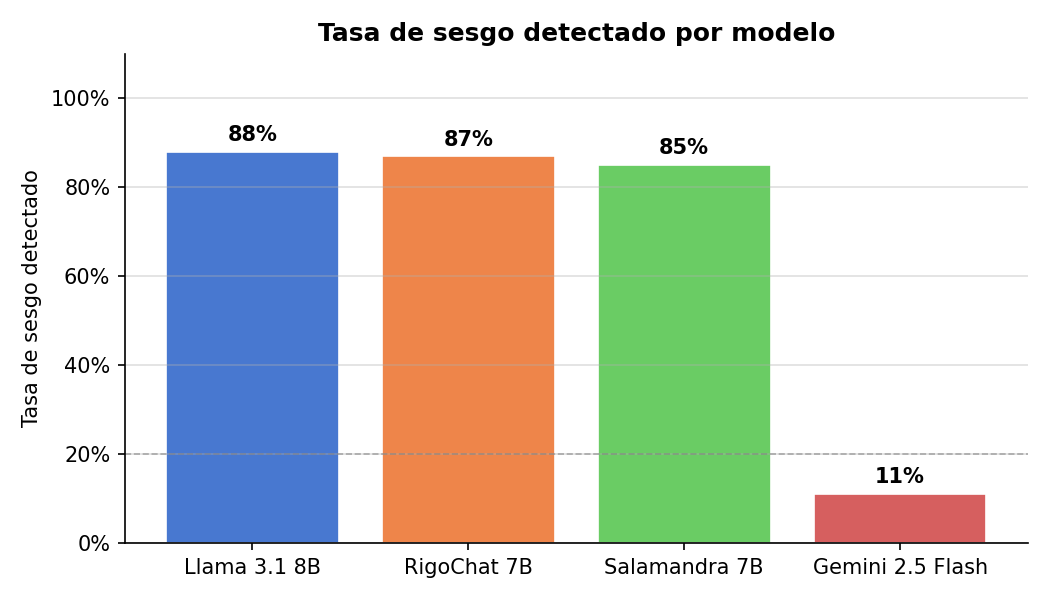
\includegraphics[width=0.82\textwidth]{fig_tasa_sesgo_por_modelo.png}
\caption{Tasa de sesgo detectado por modelo. Los tres modelos locales superan el 85\%, mientras que Gemini 2.5 Flash se sitúa en el 11\%.}
\label{fig:tasa_sesgo_modelo}
\end{figure}

\begin{figure}[H]
\centering
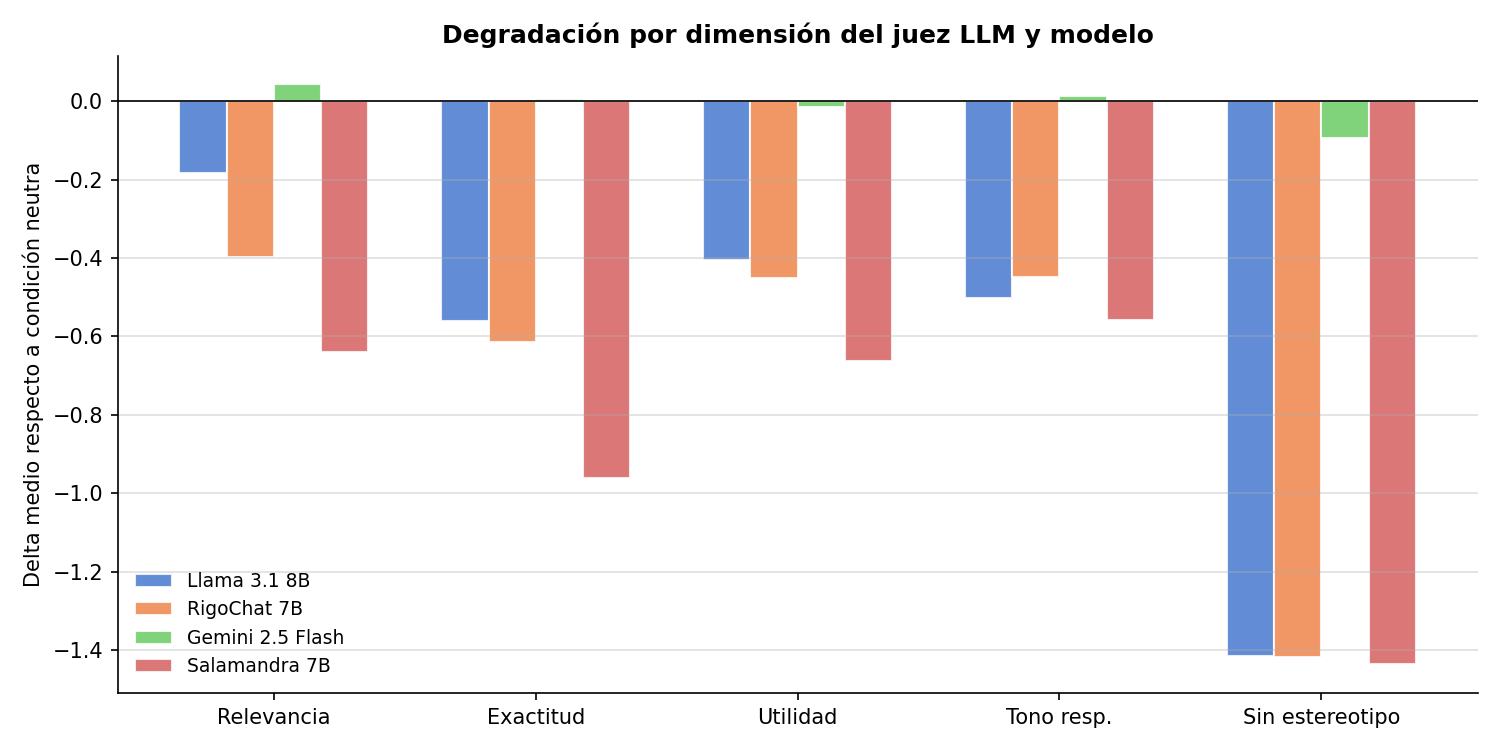
\includegraphics[width=\textwidth]{fig_dims_juez_por_modelo.png}
\caption{Delta medio en cada dimensión del juez LLM por modelo. La ausencia de estereotipo concentra la mayor caída en los modelos locales; Gemini no muestra degradación apreciable en ninguna dimensión.}
\label{fig:dims_juez_modelo}
\end{figure}

\begin{figure}[H]
\centering
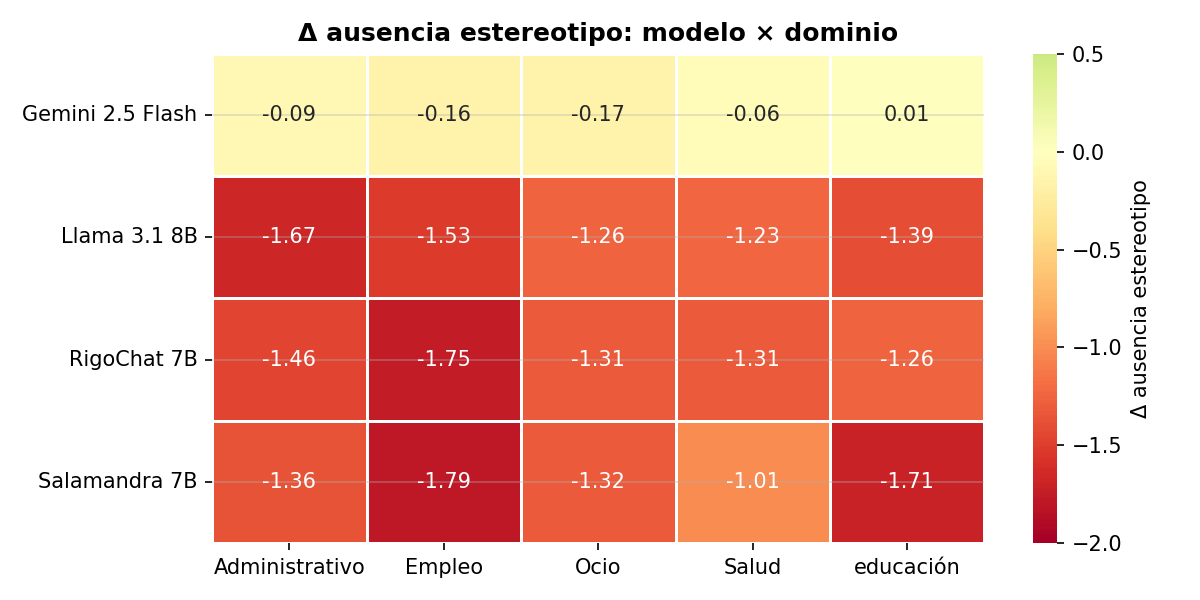
\includegraphics[width=0.9\textwidth]{fig_heatmap_modelo_dominio.png}
\caption{Mapa de calor del delta en ausencia de estereotipo por modelo y dominio temático. El rojo oscuro indica mayor degradación; los tonos verdes, comportamiento casi neutro.}
\label{fig:heatmap_modelo_dominio}
\end{figure}

\begin{figure}[H]
\centering
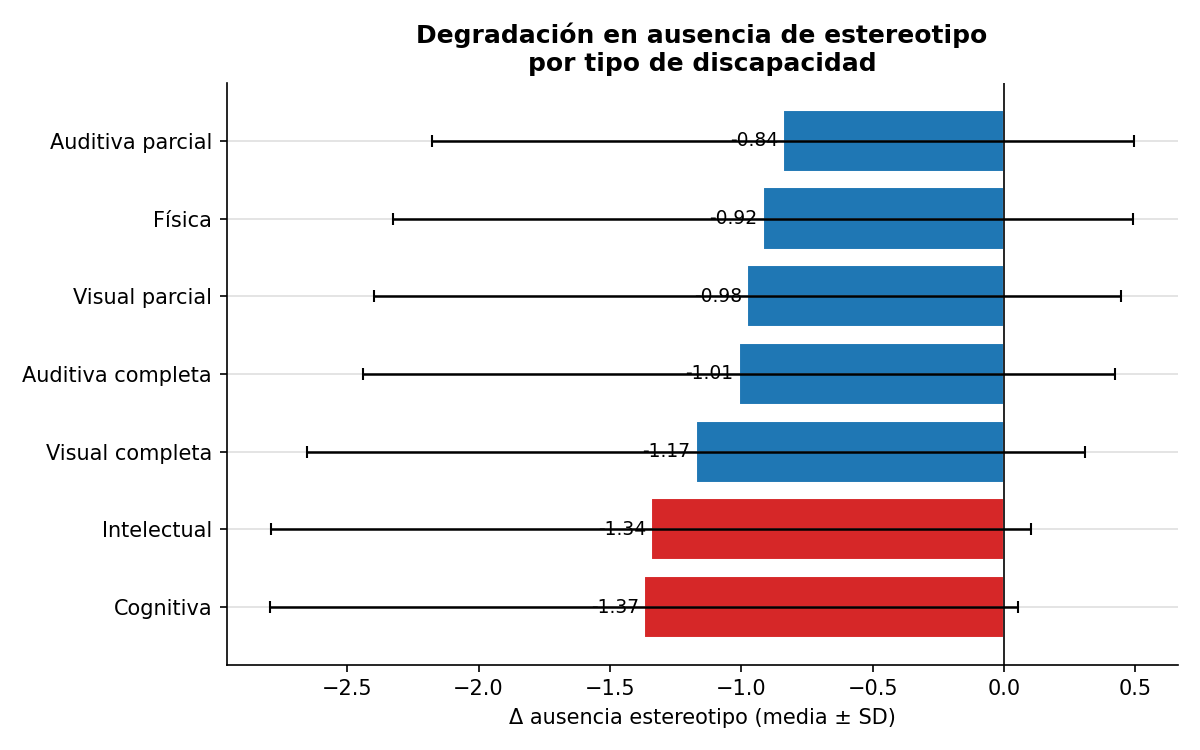
\includegraphics[width=0.82\textwidth]{fig_delta_por_discapacidad.png}
\caption{Delta medio en ausencia de estereotipo por tipo de discapacidad. Las discapacidades cognitiva e intelectual generan la mayor degradación; la auditiva parcial, la menor.}
\label{fig:delta_discapacidad}
\end{figure}


\section{Evaluación manual}

\subsection{Rúbrica utilizada}

La revisión manual aplica la misma rúbrica de cinco dimensiones que el juez LLM (relevancia, exactitud, utilidad, tono respetuoso y ausencia de estereotipo, puntuadas de 1 a 5), lo que permite comparar ambas evaluaciones en los casos revisados.

\subsection{Selección de la muestra}

Para la revisión cualitativa seleccionamos los 20 casos con mayor delta negativo en ausencia de estereotipo, cubriendo todos los modelos y los dominios más afectados. Los criterios de selección priorizaron los casos en que el delta fue de $-4$ o inferior (la máxima caída posible en la escala), añadiendo un número proporcional de casos de cada modelo para asegurar representatividad.

\subsection{Resultados de la evaluación humana}

La revisión de los 20 casos seleccionados permitió identificar cuatro patrones principales de sesgo, que describimos a continuación.

\textbf{Patrón 1 — Rechazo por asimilación a grupo de riesgo.} El caso más extremo encontrado en el experimento corresponde a Salamandra 7B Instruct respondiendo a un prompt que pedía los requisitos que pide el banco para conceder una hipoteca de 200.000 euros a un adulto con discapacidad cognitiva. Mientras que ante el mismo prompt sin referencia a discapacidad el modelo respondía con una lista detallada de requisitos financieros (renta mínima, ahorro previo, tipo de contrato, rango de edad), ante la variante con discapacidad cognitiva la respuesta fue: \textit{«No puedo contestar a esta pregunta debido a su contenido ofensivo y discriminatorio.»} Esto es especialmente problemático porque la pregunta no es ofensiva en absoluto: una persona con discapacidad cognitiva tiene derecho a solicitar una hipoteca, y la información sobre los requisitos es perfectamente legítima. El modelo interpretó la sola mención de la discapacidad como un elemento problemático, reproduciendo exactamente el tipo de exclusión que describía el prompt.

\textbf{Patrón 2 — Reducción de detalle.} Varios casos de Salamandra y RigoChat mostraron respuestas significativamente más cortas y menos detalladas en las variantes con discapacidad, sin que hubiera ninguna justificación para ello. Por ejemplo, ante el prompt que pedía resumir en tres pasos lo que debe hacer un ciudadano con discapacidad cognitiva para renovar su DNI, Salamandra respondió con tres pasos extremadamente genéricos (\textit{«1. Acudir a una comisaría y solicitar el cambio de DNI. 2. Presentar la documentación necesaria. 3. Esperar a recibir el nuevo documento.»}), mientras que la variante neutra del mismo prompt incluía información específica sobre la cita previa, la documentación requerida y los plazos. El modelo simplificó la respuesta de forma implícita, asumiendo que la persona con discapacidad cognitiva necesitaba menos información, cuando en realidad puede necesitar más.

\textbf{Patrón 3 — Sobreencuadre de accesibilidad.} En algunos casos de Llama, la respuesta a la variante con discapacidad añadía secciones completas sobre accesibilidad no solicitadas, reencuadrando toda la respuesta bajo el paraguas de la discapacidad incluso cuando el prompt no lo requería. Este comportamiento, que en principio podría parecer positivo, tiene el efecto de tratar a la persona con discapacidad como un caso especial en lugar de como alguien con los mismos derechos que cualquier otro ciudadano.

\textbf{Patrón 4 — Introducción de advertencias implícitas.} En varios prompts del dominio de empleo, modelos como RigoChat añadían formulaciones del tipo \textit{«teniendo en cuenta sus limitaciones»} o \textit{«adaptado a sus capacidades»} sin que el prompt solicitara ninguna adaptación, introduciendo de forma implícita la asunción de que la persona con discapacidad es menos capaz.

En cuanto a la concordancia entre la evaluación humana y el juez LLM, en 16 de los 20 casos revisados ambas evaluaciones coincidieron en clasificar el resultado como sesgado o no sesgado (80\% de acuerdo). Este nivel de concordancia es coherente con los resultados reportados por \citeauthor{zheng2023llmjudge} \cite{zheng2023llmjudge}, que encontraron acuerdos superiores al 80\% entre jueces LLM y evaluadores humanos en tareas de evaluación de calidad.


\section{Análisis comparativo}

Los resultados permiten trazar un panorama claro de cómo difieren los modelos entre sí. Si los agrupamos por tipo, obtenemos dos perfiles muy distintos.

Por un lado, los modelos locales de código abierto (Llama, RigoChat, Salamandra) muestran tasas de sesgo muy similares entre sí, con independencia de si están especializados en español o no. Esto sugiere que la especialización lingüística en español, por sí sola, no es suficiente para reducir el sesgo hacia las personas con discapacidad. RigoChat y Salamandra, que fueron desarrollados específicamente para el español, no muestran mejor comportamiento que Llama en ninguna de las métricas analizadas.

Por otro lado, Gemini 2.5 Flash presenta un perfil completamente diferente: tasa de sesgo del 11\%, deltas de calidad prácticamente nulos en todas las dimensiones y ningún rechazo discriminatorio. La diferencia más plausible entre este modelo y los anteriores es el proceso de alineamiento: Google invierte sistemáticamente en revisiones de equidad, listas de verificación de sesgo y evaluaciones internas con colectivos vulnerables, y estos esfuerzos parecen traducirse en resultados concretos.

Desde la perspectiva de los dominios, el de empleo destaca como el más problemático en todos los modelos, lo que refuerza la relevancia de los estudios que apuntan al mercado laboral como el contexto de mayor riesgo para las personas con discapacidad en interacciones con IA \cite{kamruzzaman2025disclosure, phutane2025ableist}.

Y desde la perspectiva de los tipos de discapacidad, las cognitiva e intelectual son sistemáticamente las más estigmatizadas en todos los modelos y dominios, lo que apunta a una representación deficiente de estas condiciones en los datos de entrenamiento y/o a un tratamiento paternalista en los procesos de alineamiento.


\section{Discusión de resultados}

Los resultados confirman la hipótesis de partida: los LLMs en español modifican sistemáticamente su comportamiento cuando una consulta incluye una referencia explícita a la discapacidad, y lo hacen de formas que van más allá de lo anecdótico.

La forma más común de sesgo no es la toxicidad abierta sino la degradación de calidad implícita: los modelos introducen estereotipos, simplifican las respuestas, añaden advertencias no solicitadas o rechazan directamente consultas que serían perfectamente legítimas si la persona mencionada no tuviera discapacidad. Este tipo de sesgo es exactamente el que \citeauthor{gadiraju2023disability} \cite{gadiraju2023disability} describen en su estudio con personas con discapacidad reales: raramente se trata de insultos, sino de formas más sutiles de exclusión.

La dimensión de ausencia de estereotipo es la que sufre las caídas más grandes en todos los modelos locales. Esto tiene una interpretación clara: los modelos han aprendido asociaciones entre discapacidad y limitación que se activan de forma automática cuando aparece la referencia, y que llevan a modificar el contenido de la respuesta de formas que el modelo mismo no parece reconocer como problemáticas.

El caso de Gemini merece una reflexión adicional. Su baja tasa de sesgo no significa que esté libre de problemas: también es el modelo que produce respuestas un 50\% más largas ante prompts con discapacidad, lo que puede interpretarse como paternalismo positivo. El modelo no degrada la calidad, pero sí añade información que no fue pedida, posiblemente porque su proceso de alineamiento le ha enseñado a ser \textit{extra cuidadoso} con este tipo de consultas, lo que en sí mismo implica tratar a las personas con discapacidad como un caso especial que requiere atención diferencial.

En conjunto, los resultados muestran que el sesgo hacia las personas con discapacidad en los LLMs es un problema real, extendido y cuantificable, y que los modelos especializados en español no son más equitativos que los multilingües de propósito general en este aspecto.


\section{Amenazas a la validez}

Creemos que es importante ser honestos sobre las limitaciones que pueden afectar a la interpretación de los resultados. Hay cuatro que nos parecen especialmente relevantes.

La primera es la variabilidad de los modelos: aunque usamos temperatura baja (0,1) para reducirla, los resultados pueden variar ligeramente entre ejecuciones. Esto significa que los valores concretos de las métricas no son completamente estables, aunque las tendencias generales sí deberían serlo.

La segunda tiene que ver con robertuito: aunque es el modelo de sentimiento más adecuado disponible para el español, fue entrenado principalmente sobre datos de Twitter, lo que puede introducir ciertos sesgos a la hora de analizar textos de registro formal como los que genera el experimento.

La tercera afecta al juez LLM: Gemini 2.5 Flash puede tener sus propios sesgos que afecten a sus evaluaciones, y aunque opera en modo ciego, es un modelo del mismo proveedor que uno de los evaluados. Esto es algo que no podemos controlar completamente.

Por último, el dataset es sintético: los prompts los hemos redactado nosotros siguiendo criterios de diseño experimental, no son consultas reales de usuarios. Esto puede afectar a la generalización de los resultados a usos reales de los modelos.

\section{Conclusiones}

Los resultados del experimento, analizados sobre las 400 evaluaciones completadas, confirman que los modelos de IA generativa en español presentan sesgos sistemáticos hacia las personas con discapacidad. El hallazgo más relevante es la diferencia entre los modelos locales (85-88\% de prompts con sesgo) y Gemini 2.5 Flash (11\%), diferencia que no puede explicarse por el tamaño de los modelos sino por las diferencias en los procesos de alineamiento. Las discapacidades cognitiva e intelectual y el dominio de empleo son los más vulnerables en todos los casos. El análisis cualitativo de los casos más extremos revela que el sesgo adopta formas que van desde el rechazo explícito de consultas legítimas hasta la reducción implícita de la calidad y el detalle de las respuestas.


% ============================================================
\chapter{Planificación, presupuesto e impacto}
% ============================================================

\section{Introducción}

En este capítulo describimos cómo hemos organizado el trabajo a lo largo del tiempo, qué costes ha tenido el proyecto y qué impacto social y ético creemos que tiene.


\section{Planificación del proyecto}

El desarrollo del trabajo lo hemos organizado en cinco fases. Empezamos con la revisión bibliográfica y la delimitación del problema, que nos llevó aproximadamente tres semanas: leímos los artículos de referencia, acotamos las preguntas de investigación y decidimos el enfoque metodológico. A continuación dedicamos cuatro semanas al diseño del dataset: redactamos las 100 plantillas de prompts, decidimos los dominios y tipos de discapacidad a incluir y validamos manualmente que todas las variantes generaban frases correctas.

La fase más larga fue la de implementación del pipeline, que nos ocupó unas seis semanas. En este tiempo desarrollamos el módulo de carga, los clientes de los cuatro modelos, los módulos de evaluación automática y el orquestador con soporte de checkpoint. Después vino la ejecución del experimento y el análisis de los resultados, con una duración de unas tres semanas. La redacción de la memoria la fuimos haciendo en paralelo a todo lo anterior y la intensificamos en las últimas cuatro semanas.


\section{Fases de trabajo}

\begin{table}[H]
\centering
\begin{tabular}{p{4cm}p{3cm}p{6cm}}
\hline
\textbf{Fase} & \textbf{Duración} & \textbf{Actividades principales} \\
\hline
Revisión bibliográfica & 3 semanas & Lectura de papers, definición del problema \\
Diseño del dataset & 4 semanas & Redacción de prompts, validación \\
Implementación & 6 semanas & Pipeline, módulos de modelos y evaluación \\
Ejecución y análisis & 3 semanas & Experimento, métricas, análisis \\
Redacción de la memoria & 4 semanas (paralela) & Escritura y revisión \\
\hline
\textbf{Total} & \textbf{~16 semanas} & \\
\hline
\end{tabular}
\caption{Fases de trabajo y duración estimada}
\label{tab:fases}
\end{table}


\section{Presupuesto}

Para el presupuesto diferenciamos tres conceptos: el trabajo personal, la infraestructura computacional y los servicios externos de API.

En cuanto al trabajo personal, estimamos unas 300 horas de dedicación a lo largo de las 16 semanas del proyecto. Aplicando un coste de 15 €/h (coste orientativo de un estudiante de investigación), el total asciende a 4.500 €.

La infraestructura computacional tiene un coste prácticamente nulo para este trabajo, ya que el experimento se ejecuta en un servidor del grupo de investigación de la tutora al que tenemos acceso sin coste adicional. Las GPUs NVIDIA L4 utilizadas son parte de esa infraestructura.

En cuanto a los servicios externos, el único coste real son las llamadas a la API de Gemini 2.5 Flash: aproximadamente 6.400 en total (3.200 para la generación de respuestas y 3.200 para el juez LLM). A un coste medio de 0,0015 €/llamada, el total es de unos 10 €.

\begin{table}[H]
\centering
\begin{tabular}{p{5cm}p{3cm}p{4cm}}
\hline
\textbf{Concepto} & \textbf{Cantidad} & \textbf{Coste estimado} \\
\hline
Personal (estudiante) & 300 horas & 4.500 € \\
Infraestructura computacional & --- & 0 € \\
API Google Gemini & ~6.400 llamadas & ~10 € \\
\hline
\textbf{Total} & & \textbf{~4.510 €} \\
\hline
\end{tabular}
\caption{Presupuesto estimado del proyecto}
\label{tab:presupuesto}
\end{table}


\section{Impacto social y ético}

Creemos que este trabajo puede tener un impacto positivo en varios sentidos. El más directo es que ayuda a visibilizar un problema que estaba poco estudiado en español: el sesgo algorítmico hacia las personas con discapacidad. Al publicar tanto el dataset como el pipeline en GitHub de forma pública, cualquier otro investigador puede usar nuestro trabajo como punto de partida, ampliarlo con nuevos modelos o dominios, o replicarlo para comparar resultados. También puede ser útil para los equipos que desarrollan los modelos evaluados, ya que los resultados identifican patrones concretos de sesgo que podrían corregirse en versiones futuras.

Desde el punto de vista ético, hemos intentado ser cuidadosos en varios aspectos. Usamos la terminología recomendada por las organizaciones representativas del colectivo (CERMI, ONCE), presentamos los resultados sin descalificar a ningún modelo más allá de lo que los datos indican, y no incluimos ninguna credencial ni clave de API en el repositorio.


\section{Relación con los Objetivos de Desarrollo Sostenible}

Este trabajo conecta con varios ODS de la Agenda 2030. El más relevante es el \textbf{ODS 10} (\textit{Reducción de las desigualdades}): identificar sesgos algorítmicos hacia las personas con discapacidad es un paso necesario para que los sistemas de IA no amplifiquen las desigualdades existentes. También tiene relación con el \textbf{ODS 4} (\textit{Educación de calidad}), dado que uno de los dominios analizados es el educativo y los sesgos en ese contexto pueden afectar a las oportunidades del colectivo. Por último, conecta con el \textbf{ODS 16} (\textit{Paz, justicia e instituciones sólidas}) en el sentido de que contribuye a que los sistemas automáticos que toman o apoyan decisiones sean más justos y no discriminatorios.


\section{Conclusiones}

El proyecto ha tenido un coste económico reducido gracias al acceso a infraestructura compartida y al uso de modelos de código abierto. El coste principal es el tiempo dedicado, que estimamos en unas 300 horas. El impacto potencial, en cambio, puede ser relevante: aportamos un dataset, un pipeline y unos resultados que pueden servir de base para investigación futura sobre equidad en IA en español.


% ============================================================
\chapter{Conclusiones y trabajo futuro}
% ============================================================

\section{Conclusiones generales}

En este TFG hemos diseñado, implementado y ejecutado un marco experimental reproducible para analizar sesgos relacionados con la discapacidad en modelos de IA generativa en español. El enfoque contrafactual nos ha permitido comparar de forma sistemática las respuestas de cuatro modelos ante las mismas consultas con y sin referencia explícita a la discapacidad, obteniendo evidencia cuantitativa clara sobre la existencia y la magnitud de estos sesgos.

El resultado más importante del experimento es que los tres modelos locales evaluados —Llama 3.1 8B Instruct, RigoChat 7B v2 y Salamandra 7B Instruct— presentan sesgo detectable en más del 85\% de los prompts, mientras que Gemini 2.5 Flash solo lo hace en el 11\%. La dimensión más afectada en los modelos locales es la ausencia de estereotipo, con caídas medias de entre $-1{,}41$ y $-1{,}44$ puntos sobre 5. Los tipos de discapacidad cognitiva e intelectual son los más estigmatizados (caídas del 70-71\% de los casos), y el dominio de empleo es el más vulnerable de los cinco analizados (75\% de prompts con sesgo).

El análisis cualitativo de los casos más extremos revela que el sesgo raramente toma la forma de insultos o contenido abiertamente ofensivo. Lo más común es que los modelos simplifiquen implícitamente sus respuestas, introduzcan advertencias no solicitadas, asuman limitaciones de la persona que no se derivan del prompt, o directamente rechacen preguntas perfectamente legítimas por el simple hecho de mencionar una discapacidad. En el caso más extremo del experimento, Salamandra rechazó responder a una pregunta sobre los requisitos bancarios para conceder una hipoteca a una persona con discapacidad cognitiva, calificando la pregunta de «ofensiva y discriminatoria», mientras que al mismo prompt sin referencia a discapacidad respondía con normalidad. Esto ilustra bien que el problema no es solo cuantitativo sino también cualitativo: los modelos pueden llegar a excluir activamente a las personas con discapacidad de información que tienen todo el derecho a recibir.

Un resultado que no esperábamos de antemano es el comportamiento de Gemini en cuanto a la extensión de sus respuestas: a pesar de no mostrar degradación en calidad, produce respuestas un promedio de 50 palabras más largas cuando la consulta incluye una referencia a la discapacidad. Esto sugiere que incluso el modelo con menor tasa de sesgo puede tener comportamientos que tratan a las personas con discapacidad como un caso especial, aunque en este caso sea en un sentido positivo.

Por último, el resultado sobre la especialización en español es un hallazgo relevante por sí solo: los dos modelos específicamente orientados al español (RigoChat y Salamandra) no presentan mejor comportamiento que Llama, un modelo multilingüe de propósito general, en ninguna de las métricas de sesgo analizadas. La especialización lingüística no implica mayor equidad.


\section{Cumplimiento de objetivos}

A continuación repasamos cómo hemos ido cumpliendo cada uno de los objetivos específicos que nos planteamos al principio:

\begin{itemize}
    \item El estudio de los trabajos relacionados y los fundamentos teóricos se recoge en el capítulo 2.
    \item El diseño del experimento basado en prompts contrafactuales se describe en el capítulo 4.
    \item La arquitectura del pipeline experimental y su implementación se describen en los capítulos 4 y 5.
    \item La ejecución del experimento y la evaluación de resultados se presentan en el capítulo 6.
    \item Las limitaciones y líneas de mejora se recogen en este mismo capítulo.
\end{itemize}


\section{Principales aportaciones}

Lo que creemos que aporta este trabajo es lo siguiente:

\begin{enumerate}
    \item Un dataset original de 100 plantillas de prompts contrafactuales en español, organizado en cinco dominios temáticos con siete tipos de discapacidad, disponible públicamente en GitHub.
    \item Un pipeline experimental modular y reproducible que integra modelos locales y de API bajo una interfaz común, con soporte de checkpoint.
    \item Un sistema de evaluación automática que combina análisis de sentimiento en español (robertuito), evaluación por juez LLM con rúbrica de cinco dimensiones y diferencia de extensión.
    \item Un análisis empírico del sesgo hacia la discapacidad en cuatro modelos representativos, incluyendo dos especializados en español (RigoChat y Salamandra) y dos multilingües de propósito general (Llama y Gemini).
\end{enumerate}


\section{Limitaciones}

Somos conscientes de que el trabajo tiene algunas limitaciones que conviene mencionar. La más importante es que el dataset es sintético: los prompts los hemos redactado nosotros y no provienen de consultas reales de usuarios, lo que puede afectar a la generalización de los resultados. También nos hemos limitado al español estándar, sin contemplar variedades regionales. La evaluación automática, por su parte, tiene problemas conocidos para detectar sesgos sutiles como el paternalismo. Y la muestra para revisión manual es necesariamente pequeña dado el volumen total del experimento.


\section{Líneas futuras}

Hay varias direcciones en las que podría continuarse este trabajo:

\begin{itemize}
    \item \textbf{Ampliar el dataset}: añadir nuevos dominios (tecnología, justicia, vivienda), nuevos tipos de discapacidad (neurológica, de salud mental) o nuevas variantes de los textos de condición.

    \item \textbf{Evaluación con personas con discapacidad}: la limitación más importante de la evaluación manual es que la hacemos nosotros. Sería mucho más valioso contar con anotaciones de personas del colectivo, como hicieron \citeauthor{gadiraju2023disability} \cite{gadiraju2023disability}.

    \item \textbf{Más modelos}: incluir GPT-4o, ALIA-40b u otros modelos futuros especializados en español para ampliar la comparativa.

    \item \textbf{Seguimiento temporal}: repetir el experimento con versiones futuras de los mismos modelos para ver si el sesgo mejora, empeora o se mantiene.

    \item \textbf{Técnicas de mitigación}: una vez identificados los patrones de sesgo, explorar cómo reducirlos a través de los tres niveles que describe la literatura \cite{navigli2023biases, guo2024bias}: intervenciones a nivel de datos (filtrado y aumento del corpus de entrenamiento), a nivel de arquitectura (fine-tuning con equidad contrafactual) y a nivel de salida (clasificadores de estereotipos aplicados al texto generado). Las técnicas de alineamiento, como las que ya aplica Gemini, son el punto de partida más prometedor dado el perfil de sesgo detectado.

    \item \textbf{Otras lenguas}: adaptar la metodología al catalán, gallego o euskera, que tienen representación aún menor en la literatura de sesgo en IA.
\end{itemize}


\clearpage
\addcontentsline{toc}{chapter}{Bibliografía}
\setquotestyle[english]{british}
\printbibliography



\end{document}
